\section{Introduction}
\label{sec:TInF-theory}

In computational wind engineering (CWE), generation of inflow turbulence satisfying prescribed mean-velocity profiles, turbulence spectra, spatial and temporal correlations is of great importance for the accurate evaluation of wind effects on buildings and structures. More specifically, the task is to generate a turbulent velocity field $\boldsymbol{u}(\boldsymbol{x},t)$ with the form

\begin{equation}
\boldsymbol{u}(\boldsymbol{x},t) = \boldsymbol{U}(\boldsymbol{x},t)+\boldsymbol{u}'(\boldsymbol{x},t)
\end{equation}

\noindent where $\boldsymbol{U}(\boldsymbol{x},t)$ and $\boldsymbol{u}'(\boldsymbol{x},t)$ are the mean and fluctuating velocities at the position $\boldsymbol{x}$. The turbulent velocity field $\boldsymbol{u}$ and its fluctuation $\boldsymbol{u}'$ need to satisfy a number of properties which are list below:

\begin{itemize}

\item $\boldsymbol{u}'$ should be spatially and temporally correlated.

\item $\boldsymbol{u}'$ needs to have prescribed Reynolds stresses tensor $R_{ij}(\boldsymbol{x}) = \langle u_i'u_j'\rangle(\boldsymbol{x})$ where $u_i'$ ($i=1,2,3$) is the $i$-th component of $\boldsymbol{u}'$  and the angles denote the time average.

\item $\boldsymbol{u}'$ needs to have prescribed integral length scales $L_{ij}(\boldsymbol{x},\boldsymbol{e})$

\begin{equation}
L_{ij}(\boldsymbol{x},\boldsymbol{e}) = \int_{0}^{\infty} \rho_{ij}(\boldsymbol{x},r\boldsymbol{e})\ \mathrm{d}r,
\end{equation}

\noindent where $\rho_{ij}(\boldsymbol{x},\boldsymbol{e})$ is the correlation function given by

\begin{equation}
\rho_{ij}(\boldsymbol{x},\boldsymbol{e}) = \frac{\langle u_i'(\boldsymbol{x},t)u_j'(\boldsymbol{x}+\boldsymbol{e},t)\rangle}{\langle u_i'(\boldsymbol{x},t)u_j'(\boldsymbol{x},t) \rangle}.
\end{equation}

\item $\boldsymbol{u}$ should fulfil the divergence free constraint $\nabla \cdot \boldsymbol{u} = 0$.

\item $\boldsymbol{u}'$ should have prescribed correlation functions $\rho_{ij}(\boldsymbol{x},\boldsymbol{e})$ or spectra.

\end{itemize}

\noindent Several methodologies have been proposed for this purpose which can be classified into three general categories: precursor simulation methods, recycling methods and synthetic methods. Compared with precursor simulation and recycling methods, the synthetic methods in general offer a more practical and relatively efficient approach to generate inflow turbulence, and is therefore chosen as the subject of this section. Research activities on synthetic turbulence generation have been vigorous over the past decades and have branched out into several categories of techniques \citep{wu2017}, including the synthetic random Fourier method \citep{kraichnan1970, hoshiya1972}, the digital filtering method \citep{klein2003, xie2008, kim2013} and the synthetic eddy methods \citep{jarrin2006, poletto2013, kroger2018}. A brief introduction regarding to these techniques is given below and emphasis is placed on their abilities to capture the statistical characteristics as well as the spatial and temporal coherence of turbulence. Also note that since real turbulence is very complex, in most cases, not all of the above listed features can be fulfilled. There is always some adaptation time required for the artificial turbulence to evolve into real turbulence. Fulfilling the properties above with the synthetic turbulence is important to minimize the adaptation time or length.

\section{Synthetic Random Fourier Method}

The so-called synthetic random Fourier method (SRFM) attempts to model turbulent flow field indirectly by imposing constraints on uncorrelated random fields through an energy spectrum to account for the spatial and temporal correlations, which can be further classified into two groups. 
The first group of the SRFM was based on the pioneering work in \cite{hoshiya1972} and \cite{shinozuka1972} on the simulation of multi-correlated random processes using a weighted amplitude wave superposition (WAWS) method. This approach has an advantage that both the targeted power- and cross-spectra can be imposed in the generation process so that the prescribed target characteristics can be maintained. A major drawback of this method is that the generated turbulence does not satisfy the continuity equation of the flow, or in other words, the divergence-free condition is not guaranteed. As a consequence it would take enormous effort for the solver to enforce the continuity by correcting the turbulence inflow inserted into the computational domain, and the statistical characteristics of the corrected flow field differs from the target values.

The second group of the SRFM was initiated by the work in \cite{kraichnan1970} on divergence-free homogeneous isotropic turbulence synthesis through the superposition of random harmonic functions. \cite{smirnov2001} took a step forward by combing Kraichnan's technique with scaling and orthogonal transformation operations in a procedure known as the random flow generation (RFG) which allows to generate inhomogeneous and anisotropic turbulence. However the scaling operation introduced in the RFG technique can result in a velocity field that is not divergence-free for inhomogeneous turbulence. Modifications to enforce the divergence-free constraint for inhomogeneous turbulence was discussed in \cite{yu2014}. A major drawback of RFG technique is that the power-spectra of the generated turbulence only follows Gaussian's spectra model, so it is not suitable for simulating flows in atmospheric boundary layer. \cite{huang2010} revisited Kraichnan's method and proposed a technique called DSRFG (for discretizing and synthesizing random flow generation) which allows to generate turbulent inflow from any prescribed spectrum. Instead of using the scaling and orthogonal transformation, the anisotropy of turbulence is realized by modifying the distribution strategy of the wave vector in Kraichnan's original method. A drawback of the DSRFG technique is that it produces fluctuating velocities with high correlation due to the fact that in this method the spatial correlation is modelled by a parameter which is not a function of frequency but a constant value. Inspired by the DSRFG method, \cite{castro2017} proposed some modifications to this technique to obtain the velocity field that had a better match with the target turbulent statistics. This method, known as modified discretizing and synthesizing random flow generation (MDSRFG), is capable of removing the dependence of statistic quantities of synthetic turbulence on spectra discretization resolution. \cite{aboshosha2015} also proposed a technique called consistent discrete RFG (CDRFG) to accurately model the target spectra and the coherence function. In both two methods mentioned above, the parameter that characterizes the spatial correlation is expressed as a function of frequency to account for the damping of coherence with the increase of frequency. An attractive feature of second group of SRFM is that the generation procedures are usually independent at each point and each time-instant so that it can be easily accelerated by conducting parallel computation, although the generated random flow may not satisfy the continuity equation. 

\section{Digital Filtering Method} \label{sectionDFM}

The digital filtering method (DFM) initiated by \cite{klein2003} attempts to model the spatial and temporal coherence of turbulent inflow through the digital filtering uncorrelated random data, and account for inhomogeneity and anisotropy using the method proposed by \cite{lund1998}. It is relatively easy to implement and is able to reproduce the first and second order one-point statistics as well as auto-correlation function. However, the synthetic turbulence generated by DFM does not satisfy the continuity equation. \cite{kim2013} offered a promising approach to enforce the divergence-free constraint in the DFM by inserting the synthetic turbulence on a transverse plane near the inlet and relying on pressure-velocity coupling to do the correction. From a computational wind engineering point of view, the ability of SDFM to impose a two-point spatial correlation directly is very attractive.

A brief introduction on the filtering method by \cite{klein2003} is stated as follows. In order to create two-point correlations, let $r_m$ be a series of random data with zero mean and unity variance, then

\begin{equation}
u_m = \sum_{n=-N}^N b_n r_{m+n}
\end{equation}

\noindent defines a convolution or a digital linear non-recursive filter. The $b_n$ are filter coefficients and $N$ is related to the length of the filter. The independence between two different random numbers $r_m$ and $r_n$ implies that $\langle r_m r_n \rangle = 0$ for $m \neq n$ and consequently the two-point correlation between $u_{m}$ and $u_{m+k}$ writes

\begin{equation} \label{SDF1}
R(k\Delta x) = \frac{\langle u_{m} u_{m+k} \rangle}{\langle u_{m} u_{m} \rangle} = \sum_{j=-N+k}^N b_j b_{j-k} / \sum_{j=-N}^N b_j^2
\end{equation}

\noindent where $\Delta x$ is the grid spacing. Note that $u_{m}$ and $u_{m+k}$ can be interpolated as the values of a random variable field (e.g., velocity) at two distinct grid points with a distance $k\Delta x$ defined on a one dimensional axis. It is straightforward to tell (\ref{SDF1}) defines a relation between the filter coefficients and the correlation function of $u_m$ (denoted by $R_{uu}$ hereafter). This suggests that a prescribed correlation function can be reproduced through a careful determination of the filter coefficients. Also note that the coefficients should be determined such that the resulting correlation function fulfil some basic properties like $R_{uu}(0)=1$, $R_{uu}(\infty) = 0$ and the prescribed integral length scales.

For a general target correlation function, the filter coefficients $b_n$ can be computed by solving a system of non-linear equations in the form of (\ref{SDF1}) with a multidimensional Newton iteration method. The procedure can be taken from a standard textbook and needs no further comment. However, for a Gaussian or an exponential type of correlation function, there exists a simple but approximate prescribed solution. More specifically, for a Gaussian correlation function in the form of

\begin{equation} \label{gaussian}
R(r) = \mathrm{exp}\left(-\frac{\pi r^2}{4L^2}\right)
\end{equation}

\noindent where $r$ is the distance and $L$ is the length scale. It is possible to approximately reproduce (\ref{gaussian}) by computing the filter coefficients as

\begin{equation}
b_k = \tilde{b}_k / \left( \sum_{j=-N}^N \tilde{b}_j^2 \right)^{1/2}
\end{equation}

\noindent where

\begin{equation}
\tilde{b}_k = e^{-\frac{\pi k^2}{2n^2}}
\end{equation}

\noindent The width $N$ of the filter should be chosen such that $N\geq 2n$ (where $n=L\Delta x_1$) to ensure the accuracy of the approximation. On the other hand, for an exponential correlation function

\begin{equation}
R(r) = \mathrm{exp}\left(-\frac{\pi |r|}{2L}\right)
\end{equation}

\noindent It is suggested by \citep{xie2008} to evaluate the filter coefficients using

\begin{equation} \label{exponential}
b_k = \tilde{b}_k / \left( \sum_{j=-N}^N \tilde{b}_j^2 \right)^{1/2}
\end{equation}

\noindent where

\begin{equation}
\tilde{b}_k = e^{-\frac{\pi|k|}{n}}
\end{equation}

\noindent Again, the width $N$ of the filter should be chosen such that $N\geq 2n$ (where $n=L\Delta x$) to ensure the accuracy of the approximation. Now we have finished the discussion of the digital filtering method for one-dimensional case. Such a technique of generating spatially (or temporally) correlated data from general random numbers can be easily extended to three dimensional case by introducing multi-index filter coefficients $b_{ijk}$ defined as

\begin{equation}
b(i,j,k) = b_{ijk} = b_i \cdot b_j \cdot b_k
\end{equation}

\noindent An algorithm for generating inflow data may look like this (alternatively one can generate a large volume of data, store it and convect it through the inflow plane by applying Taylor's hypothesis):

\begin{enumerate}[(a)]

\item Choose for each coordinate direction corresponding to the inflow plane a length scale $L_{22} = n_2\Delta x_2$, $L_{33} = n_3\Delta x_3$, a time scale $T$ and determine the filter width $N_{\alpha}$ ($\alpha =1,2,3$) accordingly.

\item Initialize and store three random fields $R_{\alpha}$ (again $\alpha =1,2,3$) of dimensions $[-N_1:N_1,-N_2+1:M_2+N_2,-N_3+1:M_3+N_3]$ where $M_2 \times M_3$ denotes the dimensions of computational gird of the inflow plane.

\item Compute the filter coefficients $b(i,j,k)$ with a prescribed function or by a multidimensional Newton method such that the resulting correlation function (\ref{SDF1}) meets the target one.

\item Applying the following filter operation for $j=1,\ldots,M_2$, $k=1,\ldots,M_3$

\begin{equation}
\Psi_{\alpha}(j,k) = \sum_{i'=-N_1}^{N_1}\sum_{j'=-N_2}^{N_2}\sum_{k'=-N_3}^{N_3}b(i',j',k')R_{\alpha}(i',j+j',k+k')
\end{equation}

\noindent which yields the two-dimensional arrays of spatially correlated data $\Psi_{\alpha}$, $\alpha =1,2,3$.

\item Output velocity data with the transformation

\begin{equation}
u_i(j,k) = U_i + a_{ij}\Psi_j(j,k)
\end{equation}

\noindent where the coefficients $a_{ij}$ are given by (\ref{LundCoefficients}). This step ensures the synthetic velocity reproduces the target mean velocity and Reynolds stress tensor.

\item Discard the first $(x_2,x_3)$-plane of $\Psi_{\alpha}$ and shift the whole data: $\Psi_{\alpha}(i,j,k)\coloneqq R_{\alpha}(i+1,j,k)$. Fill the plane $R_{\alpha}(N_1,j,k)$ with new random numbers.

\item Repeat the steps (d)$\sim$(g) for each time step.

\end{enumerate}

If the target correlation function is an exponential function, an alternative approach by \cite{xie2008} can be adopted for generating inflow turbulence which turns out to be much more efficient than the method of \cite{klein2003}. Instead of using the filtering operation discussed above, the method of \cite{xie2008} obtain the temporal correlation with the expression

\begin{equation} \label{temporalCorrelation}
\Psi_{\alpha}(t+\Delta t,j,k) = \Psi_{\alpha}(t,j,k)\mathrm{exp}\left(-\frac{\pi \Delta t}{2T} \right)+\varPsi_{\alpha}(t,j,k)\left[1-\mathrm{exp}\left(-\frac{\pi \Delta t}{T} \right)\right]^{0.5}
\end{equation}

\noindent where $\Psi_{\alpha}(t,j,k)$ and $\varPsi_{\alpha}(t,j,k)$ are two set of spatially-correlated random data resulting from a two dimensional filtering operation. For simplicity, we write $\Psi_{\alpha,0}$, $\Psi_{\alpha,k}$, $\varPsi_{\alpha,0}$ and $\varPsi_{\alpha,k}$ for $\Psi_{\alpha}(t,j,k)$, $\Psi_{\alpha}(t+k\Delta t,j,k)$, $\varPsi_{\alpha}(t,j,k)$ and $\varPsi_{\alpha}(t+k\Delta t,j,k)$, respectively. One easily verifies that

\begin{equation}
\begin{split}
\left\langle \Psi_{\alpha,0}\Psi_{\alpha,k} \right\rangle &= \left\langle \Psi_{\alpha,0}\left\{\Psi_{\alpha,k-1}\left(-\frac{\pi \Delta t}{2T} \right)+ \varPsi_{\alpha,k-1}\left[1-\mathrm{exp}\left(-\frac{\pi \Delta t}{T} \right)\right]^{0.5}\right\}\right\rangle \\
& = \left\langle \Psi_{\alpha,0} \Psi_{\alpha,k-1} \right\rangle \mathrm{exp}\left(-\frac{\pi \Delta t}{2T}\right) \\
& \cdots \\
& = \mathrm{exp}\left(-\frac{k\pi \Delta t}{2T}\right)
\end{split}
\end{equation}

\noindent which reproduces an exponential function. An overall algorithm for generating the inflow velocity supported by the method of \cite{xie2008} can be stated as follows

\begin{enumerate}[(a)]

\item Choose for each coordinate direction corresponding to the inflow plane a length scale $L_{22} = n_2\Delta x_2$, $L_{33} = n_3\Delta x_3$, a time scale $T$ and determine the filter width $N_{\alpha}$ ($\alpha = 1,2,3$) accordingly.

\item Initialize and store three random fields $R_{\alpha}$ (again $\alpha =1,2,3$) of dimensions $[-N_2+1:M_2+N_2,-N_3+1:M_3+N_3]$ where $M_2 \times M_3$ denotes the dimensions of computational gird in the inflow plane.

\item Compute the filter coefficients $b(j,k)$ with a prescribed function or by a multidimensional Newton method such that the resulting correlation function meet the target one.

\item Applying the following filter operations for $j=1,\ldots,M_2$, $k=1,\ldots,M_3$

\begin{equation}
\varPsi_{\alpha}(j,k) = \sum_{j'=-N_2}^{N_2}\sum_{k'=-N_3}^{N_3}b(j',k')R_{\alpha}(j+j',k+k')
\end{equation}

\noindent which yields the two-dimensional arrays of spatially correlated data $\varPsi_{\alpha}$, $\alpha =1,2,3$.

\item Compute $\Psi_{\alpha}(j,k)$ with (\ref{temporalCorrelation}) and output the velocity signal with the transformation

\begin{equation}
u_i(j,k) = U_i + a_{ij}\Psi_j(j,k)
\end{equation}

\noindent where the coefficients $a_{ij}$ are given by (\ref{LundCoefficients}). Again, this step ensures the synthetic velocity reproduces the target mean velocity and Reynolds stress tensor.

\item Repeat the steps (d)$\sim$(f) for each time step.

\end{enumerate}


\section{Synthetic Eddy Method}\label{sectionSEM}

The synthetic eddy method (SEM) initiated by \cite{jarrin2006} is based on the classical view of turbulence as a superposition of the representative coherent eddies. In the SEM, the flow is assumed to consist of randomly distributed turbulent spots, and each turbulent spot is modelled by a three-dimensional shape function with compact support and satisfies a proper normalization condition. The spots are then assumed to be convected through an inlet plane with a reference velocity using Taylor's frozen turbulence hypothesis. The resulting inflow turbulence is then reconstructed using the method proposed by to recover the desired statistical characteristics and to account for the conditions of inhomogeneity and anisotropy. The choice of the shape function plays an important role in the SEM since it is directly related to the two-point auto-correlation function, and consequently the power spectrum of the synthetic turbulence. Enforcement of the continuity condition in the SEM was discussed in \cite{poletto2013} which will be introduced later.

A brief introduction on the SEM presented by \cite{jarrin2006} is given as follows. To start with, the turbulent spot mentioned above can be represented as eddies defined by shape function $f$ which has a compact support on $[-1,1]$ and has the normalization

\begin{equation} \label{normalization}
\int_{-1}^1 f^2(x) \mathrm{d}x = 1
\end{equation}

\noindent The inflow plane on which we want to generate the synthetic turbulence with the SEM is basically a finite set of points $S = \{\boldsymbol{x}_1,\boldsymbol{x}_2,\ldots,\boldsymbol{x}_s\}$. The first step is to create a box of eddies $B$ surrounding $S$ which is going to contain the synthetic eddies. It is defined by

\begin{equation}
B = \big\{(x_1,x_2,x_3)\in \mathbb{R}^3: x_{i,\text{min}}<x_i<x_{i,\text{max}}\big\}
\end{equation}

\noindent where

\begin{equation}
x_{i,\text{min}} = \text{min}(x_i-\sigma_i(\boldsymbol{x})), \quad x_{i,\text{max}} = \text{max}(x_i+\sigma_i(\boldsymbol{x})), \quad \boldsymbol{x}\in S
\end{equation}

\noindent The volume of the box of eddies is noted by $V_B$. In the synthetic eddy method, the velocity signal generated by $N$ eddies has the representation

\begin{equation} \label{SEMvelocity}
u_i(\boldsymbol{x}) = U_i(\boldsymbol{x}) + \frac{1}{\sqrt{N}}\sum_{k=1}^N a_{ij} \epsilon_j^k f_{\boldsymbol{\sigma}(\boldsymbol{x})}(\boldsymbol{x}-\boldsymbol{x}^k)
\end{equation}

\noindent where $\boldsymbol{x}$ represent the coordinates of computational points and $\boldsymbol{x}^k$ represent the coordinates of eddies. The coefficient $a_{ij}$ results from the Cholesky decomposition of a prescribed Reynolds stress tensor $R_{ij}$

\begin{equation} \label{LundCoefficients}
\left(\begin{matrix}
\sqrt{R_{11}} & 0 & 0 \\
R_{21}/a_{11} & \sqrt{R_{22}-a_{21}^2} & 0 \\
R_{31}/a_{11}  & (R_{32}-a_{21}a_{31})/a_{22} & \sqrt{R_{33}-a_{31}^2--a_{32}^2}
\end{matrix}\right)
\end{equation}

\noindent The coefficient $\epsilon_j^k$ ($j=1,2,3$) is is the uniformly random intensity factor of values $+1$ or $-1$, and $f_{\boldsymbol{\sigma}(\boldsymbol{x})} (\boldsymbol{x}-\boldsymbol{x}^k)$ is the velocity distribution at $\boldsymbol{x}$ of the eddy located at $\boldsymbol{x}^k$ defined as follows:

\begin{equation} \label{eddyType}
f_{\boldsymbol{\sigma}(\boldsymbol{x})} (\boldsymbol{x}-\boldsymbol{x}^k) = \sqrt{\frac{V_B}{\sigma_1\sigma_2\sigma_3}}f\left(\frac{x_1-x_1^k}{\sigma_1}\right)f\left(\frac{x_2-x_2^k}{\sigma_2}\right)f\left(\frac{x_3-x_3^k}{\sigma_3}\right)
\end{equation}

\noindent where $\boldsymbol{\sigma}=(\sigma_1,\sigma_2,\sigma_3)^T$. The position of the eddies $\boldsymbol{x}^k$ before the first time step are independent from each other and taken from a uniform distribution over the box of eddies $B$. The eddies are convected through the box of eddies $B$ with the mean velocity $\boldsymbol{U}(\boldsymbol{x})$. At each time step, the new position of eddy $k$ is given by

\begin{equation}
\boldsymbol{x}^k(t+\Delta t) = \boldsymbol{x}^k(t)+\boldsymbol{U}(\boldsymbol{x}^k)\Delta t
\end{equation}

\noindent where $\Delta t$ is the time step of the simulation. If an eddy $k$ is convected out of the box $B$, then it is immediately regenerated randomly with in the region

\begin{equation}
B_{\Delta t} = \left\{ \boldsymbol{x}\notin B, \ \boldsymbol{x}+\boldsymbol{U}(\boldsymbol{x})\Delta t \in B \right\}
\end{equation}

\noindent with a new random intensity vector $\epsilon_j^k$. $B_{\Delta t}$ denotes the region in which regenerated eddy $\boldsymbol{x}^k(t) \in B_{\Delta t}$ dose not effect the synthetic velocity at the inflow plane until the next time-step.

\subsection{Mean flow and Reynolds stresses}

\noindent The mean value of the velocity signal (\ref{SEMvelocity}) can be expressed as

\begin{equation}
\left\langle u_i \right\rangle = U_i(\boldsymbol{x}) + \frac{1}{\sqrt{N}}\sum_{k=1}^N \left\langle a_{ij} \varepsilon_j^k f_{\boldsymbol{\sigma}(\boldsymbol{x})}(\boldsymbol{x}-\boldsymbol{x}^k) \right\rangle
\end{equation}

\noindent The independence between the random variables $\boldsymbol{x}^k$ and $\varepsilon_j^k$ in the mean operator implies that

\begin{equation}
\left\langle a_{ij} \varepsilon_j^k f_{\boldsymbol{\sigma}(\boldsymbol{x})}(\boldsymbol{x}-\boldsymbol{x}^k) \right\rangle = a_{ij} \left\langle\varepsilon_j^k\right\rangle  \left\langle f_{\boldsymbol{\sigma}(\boldsymbol{x})}(\boldsymbol{x}-\boldsymbol{x}^k)  \right\rangle
\end{equation}

\noindent The term $\langle\varepsilon_j^k\rangle = 0$ since the intensities of the eddies is either $1$ or $-1$ with equal probability. Consequently, we obtain

\begin{equation}
\left\langle u_i \right\rangle = U_i(\boldsymbol{x}).
\end{equation}

\noindent The Reynolds stresses $\langle u_i u_j \rangle$ of the synthesized write

\begin{equation}
\langle u_i' u_j' \rangle = \frac{1}{N}\sum_{k=1}^N\sum_{k=1}^N a_{im}a_{jn} \langle \varepsilon_m^k \varepsilon_n^l \rangle \langle f_{\boldsymbol{\sigma}(\boldsymbol{x})}(\boldsymbol{x}-\boldsymbol{x}^k) f_{\boldsymbol{\sigma}(\boldsymbol{x})}(\boldsymbol{x}-\boldsymbol{x}^l) \rangle
\end{equation}

\noindent Using again the independence between the random variables $\boldsymbol{x}^k$ and $\varepsilon_j^k$, the above equation reduces to

\begin{equation}
\langle u_i' u_j' \rangle = \frac{1}{N}\sum_{k=1}^N a_{im}a_{jm} \langle f_{\boldsymbol{\sigma}(\boldsymbol{x})}^2(\boldsymbol{x}-\boldsymbol{x}^k)
\end{equation}

\noindent The term

\begin{equation}
\langle f_{\boldsymbol{\sigma}(\boldsymbol{x})}^2(\boldsymbol{x}-\boldsymbol{x}^k) \rangle = \int_{\mathbb{R}^3} p(\boldsymbol{y}) f_{\boldsymbol{\sigma}(\boldsymbol{x})}^2(\boldsymbol{x}-\boldsymbol{x}^k) = 1
\end{equation}

\noindent follows from the fact that $\boldsymbol{x}^k$ follows a uniform distribution over $B$, i.e. 

\begin{equation} \label{distribution}
p(\boldsymbol{y}) = 
\begin{cases}
\frac{1}{V_B} & \boldsymbol{y} \in B \\
0 & \boldsymbol{y} \notin B
\end{cases}.
\end{equation}

\noindent Finally, we arrive at

\begin{equation} \label{ReynoldsStresses}
\langle u_i u_j \rangle = \frac{1}{N}\sum_{k=1}^N a_{im}a_{jm} = R_{ij}
\end{equation}

\noindent Hence the Reynolds stresses of the velocity fluctuations generated by the SEM reproduce exactly the input Reynolds stresses.

\subsection{Two-point correlation}

\noindent The two-point cross-correlation of the velocity fluctuations writes

\begin{equation} \label{twoPointCorrelations0}
R_{ij}(\boldsymbol{x},\boldsymbol{r}) = \langle u_i(\boldsymbol{x},t) u_j(\boldsymbol{x}+\boldsymbol{r},t) \rangle
\end{equation}

\noindent where $\boldsymbol{r} = (r_1,r_2,r_3)$ is a vector defining the relative positions between the two points at which the velocity correlations are computed. By (\ref{SEMvelocity}) and the linearity of the statistical mean, we obtain

\begin{equation}
R_{ij}(\boldsymbol{x},\boldsymbol{r}) = \frac{1}{N}\sum_{k=1}^N\sum_{k=1}^N a_{im}a_{jn} \langle \varepsilon_m^k \varepsilon_n^l \rangle \langle f_{\boldsymbol{\sigma}(\boldsymbol{x})}(\boldsymbol{x}-\boldsymbol{x}^k) f_{\boldsymbol{\sigma}(\boldsymbol{x}+\boldsymbol{r})}(\boldsymbol{x}+\boldsymbol{r}-\boldsymbol{x}^l) \rangle 
\end{equation}

\noindent Using again the independence between the positions $\boldsymbol{x}^k$ and the intensities $\varepsilon^k$ of the eddies, this yields

\begin{equation} \label{twoPointCorrelations1}
R_{ij}(\boldsymbol{x},\boldsymbol{r}) = \frac{1}{N}\sum_{k=1}^N a_{im}a_{jm} \langle f_{\boldsymbol{\sigma}(\boldsymbol{x})}(\boldsymbol{x}-\boldsymbol{x}^k) f_{\boldsymbol{\sigma}(\boldsymbol{x}+\boldsymbol{r})}(\boldsymbol{x}+\boldsymbol{r}-\boldsymbol{x}^k) \rangle 
\end{equation}

\noindent By (\ref{distribution}), the term in the mean operator writes

\begin{equation} \label{twoPointCorrelations2}
\langle f_{\boldsymbol{\sigma}(\boldsymbol{x})}(\boldsymbol{x}-\boldsymbol{x}^k) f_{\boldsymbol{\sigma}(\boldsymbol{x}+\boldsymbol{r})}(\boldsymbol{x}+\boldsymbol{r}-\boldsymbol{x}^k) \rangle = \frac{1}{V_B} \int_B f_{\boldsymbol{\sigma}(\boldsymbol{x})}(\boldsymbol{x}-\boldsymbol{y}) f_{\boldsymbol{\sigma}(\boldsymbol{x}+\boldsymbol{r})}(\boldsymbol{x}+\boldsymbol{r}-\boldsymbol{y}) \mathrm{d}\boldsymbol{y}
\end{equation}

\noindent Inserting (\ref{twoPointCorrelations2}) back to (\ref{twoPointCorrelations1}) and using (\ref{eddyType}), this yields

\begin{equation} \label{twoPointCorrelations3}
R_{ij}(\boldsymbol{x},\boldsymbol{r}) = R_{ij} \cdot \prod_{l=1}^3 \left[f_{\boldsymbol{\sigma}(\boldsymbol{x})} *f_{\boldsymbol{\sigma}(\boldsymbol{x}+\boldsymbol{r})} \right](r_l)
\end{equation}

\noindent where $\*$ denotes the convolution product. For homogeneous turbulence where integral length scales $\boldsymbol{\sigma}(\boldsymbol{x}) = \boldsymbol{\sigma}(\boldsymbol{x}+\boldsymbol{r}) =(\sigma,\sigma,\sigma)^T$, the two-point cross-correlation tensor $R_{ij}(\boldsymbol{x},\boldsymbol{r})$ only depends on $\boldsymbol{r}$ and consequently (\ref{twoPointCorrelations3}) simplifies to 

\begin{equation} \label{twoPointCorrelations4}
R_{ij}(\boldsymbol{r}) = R_{ij} \cdot \prod_{l=1}^3 \left[f*f\right]\left(\frac{r_l}{\sigma}\right)
\end{equation}

\noindent Recall the integral length scale $L_{ij}$ is defined as the integral of the two-point correlation $R_{ij}(\boldsymbol{x},\boldsymbol{r})$ in a particular direction and is thus proportional to $\sigma$. By integrating (\ref{twoPointCorrelations4}), one easily verifies that (for homogeneous turbulence) $L_{ij}=C_f\sigma$ in every direction where $C_f$ only depends on the choice of $f$. 

Fourier analysis can also be used to obtain the spectra of the synthetic turbulence. Note that the velocity spectrum tensor $\phi_{ij}(k)$ is the Fourier transform of the two-point correlation tensor 

\begin{equation}
\phi_{ij}(\boldsymbol{k}) = \mathcal{F}_{\boldsymbol{k}}\left\{R_{ij}(\boldsymbol{r})\right\}
\end{equation}

\noindent Recall the convolution theorem for cross-correlation states that 

\begin{equation}
\mathcal{F}_{\boldsymbol{k}}\left\{f * f\right\} = |\mathcal{F}_{\boldsymbol{k}}\left\{f\right\}|^2
\end{equation}

\noindent Hence the spatial velocity spectrum tensor can be expressed as

\begin{equation}
\phi_{ij}(\boldsymbol{k}) = R_{ij}\sigma^3 \cdot \prod_{l=1}^3|\mathcal{F}_{k_l\sigma}\left\{f\right\}|^2
\end{equation}

\noindent where $\boldsymbol{k} = (k_1,k_2,k_3)$. More specifically for instance, the one-dimensional spectra in the $x$ direction is

\begin{equation}
E_{ij}(k) = R_{ij}\sigma^3 \cdot |\mathcal{F}_{k_l\sigma}\left\{f\right\}|^2
\end{equation}

\subsection{Two-time correlation}

The two-time correlation tensor of the velocity, denoted by $R_{ij}(\boldsymbol{x},\tau)$, is the correlation between $u_i(\boldsymbol{x},t)$ and $u_j(\boldsymbol{x},t+\tau)$ at times $t$ and $t+\tau$ respectively, i.e.,

\begin{equation} \label{twoTimeCorrelation0}
R_{ij}(\boldsymbol{x},\tau) = \langle u_i'(\boldsymbol{x},t) u_j'(\boldsymbol{x},t+\tau) \rangle.
\end{equation}

\noindent By (\ref{SEMvelocity}) and the linearity of the statistical mean, we have

\begin{equation} \label{twoTimeCorrelation1}
R_{ij}(\boldsymbol{x},\tau) = \frac{1}{N}\sum_{k=1}^N\sum_{k=1}^N a_{im}a_{jn} \langle \varepsilon_m^k(t) \varepsilon_n^l(t+\tau) f_{\boldsymbol{\sigma}(\boldsymbol{x})}(\boldsymbol{x}-\boldsymbol{x}^k(t)) f_{\boldsymbol{\sigma}(\boldsymbol{x})}(\boldsymbol{x}-\boldsymbol{x}^l(t+\tau)) \rangle 
\end{equation}

\noindent The independence between the position $\boldsymbol{x}^k$ and intensity $\varepsilon_m^k$ of different eddies implies that, for $k \neq l$, the statistical mean in (\ref{twoTimeCorrelation1}) can be split as follows

\begin{equation}
\langle \varepsilon_m^k(t) \rangle \langle \varepsilon_n^l(t+\tau) \rangle \langle f_{\boldsymbol{\sigma}(\boldsymbol{x})}(\boldsymbol{x}-\boldsymbol{x}^k(t)) \rangle \langle f_{\boldsymbol{\sigma}(\boldsymbol{x})}(\boldsymbol{x}-\boldsymbol{x}^l(t+\tau)) \rangle = 0
\end{equation}

\noindent Consequently (\ref{twoTimeCorrelation1}) reduces to

\begin{equation} \label{twoTimeCorrelation2}
R_{ij}(\boldsymbol{x},\tau) = \frac{1}{N}\sum_{k=1}^N a_{im}a_{jn} \langle \varepsilon_m^k(t) \varepsilon_n^k(t+\tau) f_{\boldsymbol{\sigma}(\boldsymbol{x})}(\boldsymbol{x}-\boldsymbol{x}^k(t)) f_{\boldsymbol{\sigma}(\boldsymbol{x})}(\boldsymbol{x}-\boldsymbol{x}^k(t+\tau)) \rangle 
\end{equation}

\noindent Before computing the term in the angles, we define $B_{\tau} \in B$  such that all eddies that present in $B_{\tau}$ at time $t$ will be convected far enough so that they will be recycled at least once before time $t+\tau$

\begin{equation}
B_{\tau} = \left\{\boldsymbol{x}\in B, \ \boldsymbol{x}+\tau \boldsymbol{U}(\boldsymbol{x}) \in B \right\}
\end{equation}

\noindent If $\boldsymbol{x}^k(t)\in B_{\tau}$, then it is going to be recycled between time $t$ and $t+\tau$ and hence both $\boldsymbol{x}^k(t+\tau)$ and $\varepsilon_m^k(t+\tau)$ will be independent of their previous values. The contribution of an eddy $k$ located within the region where $\boldsymbol{x}^k(t) \in B_{\tau}$ to the term in the angles of (\ref{twoTimeCorrelation2}) is thus zero. On the contrary if $\boldsymbol{x}^k(t) \in B_{\tau}$, the eddy $k$ will remain inside of the box $B$ at time $t + \tau$ and hence $\varepsilon_m^k(t+\tau) =  \varepsilon_m^k(t)$ and $\boldsymbol{x}^k(t+\tau) =\boldsymbol{x}^k(t)+\tau\boldsymbol{U}(\boldsymbol{x}^k)$. Thus both $\varepsilon_n^k(t+\tau) =  \varepsilon_n^k(t)$ and $\boldsymbol{x}^k(t+\tau)$ depend on the previous position $\boldsymbol{x}^k(t)$ of eddy $k$ relative to $B_{\tau}$. By (\ref{ReynoldsStresses}) and the definition of $B_{\tau}$, (\ref{twoPointCorrelations0}) can then be replaced by

\begin{equation} \label{twoTimeCorrelation3}
R_{ij}(\boldsymbol{x},\tau) = R_{ij} \int_{B/B_{\tau}}f_{\boldsymbol{\sigma}(\boldsymbol{x})}(\boldsymbol{x}-\boldsymbol{y}) f_{\boldsymbol{\sigma}(\boldsymbol{x})}(\boldsymbol{x}-(\boldsymbol{y}+\tau\boldsymbol{U}_c)) \ \mathrm{d}\boldsymbol{y}
\end{equation}

\noindent The condition $\boldsymbol{y}\in B_{\tau}$ leads to $f_{\boldsymbol{\sigma}(\boldsymbol{x})}(\boldsymbol{x}-(\boldsymbol{y}+\tau\boldsymbol{U}))=0$. Thus, the integral over $B/B_{\tau}$ in (\ref{twoPointCorrelations3}) can be extended to an integral over $B$. Besides $\boldsymbol{y}\in B$ suggests $f_{\boldsymbol{\sigma}(\boldsymbol{x})}(\boldsymbol{x}-\boldsymbol{y})=0$ as previously demonstrated, therefore the integral in (\ref{twoTimeCorrelation3}) can be further extended to an integral over $\mathbb{R}^3$. Using (\ref{eddyType}), this yields

\begin{equation} \label{twoTimeCorrelation4}
R_{ij}(\boldsymbol{x},\tau) = R_{ij} \cdot \prod_{l=1}^3[f*f]\left(\frac{\tau U_{l}(\boldsymbol{x})}{\sigma_l(\boldsymbol{x})}\right)
\end{equation}

\noindent In the case where the mean velocity is in the $x_1$-direction only $\boldsymbol{U} = (U,0,0)$ and the target turbulence is homogeneous, (\ref{twoTimeCorrelation4}) simplifies to

\begin{equation}
R_{ij}(\boldsymbol{x},\tau) = R_{ij} [f*f]\left(\frac{\tau U(\boldsymbol{x})}{\sigma(\boldsymbol{x})}\right)
\end{equation}

\noindent Thus, the two-time correlation of the signal at time $\tau$ is simply the auto-correlation function of $f$ at separation distance $\tau U /\sigma$. By integrating the above equation it can be proved that the integral time scale of the signal writes $T = \sigma/U C_f$ where $C_f$ is a coefficient only depends on the choice of $f$. Since the synthetic velocity is a stationary process, the information the two-time cross-correlation tensor $R_{ij}(\boldsymbol{x},\tau)$ contains can be re-expressed in terms of the wave number velocity spectrum tensor which writes

\begin{equation}
\phi_{ij}(\boldsymbol{x},\omega) = \mathcal{F}_{\omega}\{R_{ij}(\boldsymbol{x},\tau)\}
\end{equation}

\noindent Using again the convolution theorem, the above expression simplifies to

\begin{equation}
\phi_{ij}(\boldsymbol{x},\omega) = R_{ij}\frac{\sigma}{|U|} |\mathcal{F}_{\omega\sigma / |U|}\{f\}|^2
\end{equation}

\subsection{Commonly used velocity shape functions}

The three commonly used velocity shape functions for $f$ are given below for reference which are the tent function, the step function and the truncated Gaussian function.

\begin{itemize}
\item Tent function

\begin{equation}\label{ftent}
f(x) =
\begin{cases}
\sqrt{\frac{3}{2}}(1-|x|), & 0 \leq |x| < 1 \\
0, & |x| \geq 1
\end{cases}
\end{equation}

\begin{equation}
[f*f](r) = 
\begin{cases}
1-\frac{3}{2}r^2+\frac{3}{4}|r|^3, & 0 \leq |r| < 1 \\
2-3|r|+\frac{3}{2}r^2-\frac{1}{4}|r|^3, & 1 \leq |r| <2 \\
0, & |r|\geq 2
\end{cases}
\end{equation}

\item Step function

\begin{equation}\label{fstep}
f(x) =
\begin{cases}
\frac{1}{\sqrt{2}}, & 0 \leq |x| < 1 \\
0, & |x| \geq 1
\end{cases}
\end{equation}

\begin{equation}
[f*f](r) = 
\begin{cases}
1-\frac{|r|}{2}, & 0 \leq |r| < 2 \\
0, & |r|\geq 2
\end{cases}
\end{equation}

\item Truncated Gaussian function

\begin{equation}\label{fgaussian}
f(x) =
\begin{cases}
Ce^{-9x^2/2}, & 0 \leq |x| < 1 \\
0, & |x| \geq 1
\end{cases}
\end{equation}

\begin{equation}
[f*f](r) = 
\begin{cases}
e^{-9r^2/4} & 0\leq |r| < 2 \\
0, & |r|\geq 2
\end{cases}
\end{equation}

\noindent where $C$ is a constant that ensures $f$ satisfies the normalization (\ref{normalization}).

\end{itemize}

\section{Divergence Free Synthetic Eddy Method}

One route to obtain a divergence free method, as suggested by \cite{poletto2013}, is to apply the original SEM methodology to the vorticity field, which is then transformed back to the velocity field by taking the curl of it. One easily verifies that vorticity and velocity fields are linked by the following:

\begin{equation}
	\nabla\times\omega' = \nabla(\nabla\cdot\boldsymbol{u}')-\nabla^2\boldsymbol{u}'
\end{equation}

\noindent Because of the hypothesis of incompressible flow, the first term on the right hand side of the above equation vanishes, leading to a Poisson equation for the velocity field. The solution of this Poisson equation, achieved by using the Biot–Savart kernel, leads to the fluctuating velocity field expressed as:

\begin{equation} \label{DFSEMvelocity}
	\boldsymbol{u}'(\boldsymbol{x}) = \sqrt{\frac{1}{N}}\sum_{k=1}^N\frac{q_{\sigma}(|\boldsymbol{r}^k|)}{|\boldsymbol{r}^k|}\boldsymbol{r}^k\times\alpha^k
\end{equation}

\noindent where $\boldsymbol{r}^k=(\boldsymbol{x}-\boldsymbol{x}^k)/\sigma^k$, $q_{\sigma}(|\boldsymbol{r}^k|)$ is a suitable shape function and $\alpha_i^k$ are random numbers with zero average which represent the eddy intensities.

Despite the similarities between (\ref{SEMvelocity}) and (\ref{DFSEMvelocity}), i.e. both including a user defined shape function and a random level eddy intensity, the lack of Lund coefficients in the second formulation poses a significant problem. Their role in the original SEM was crucial in order to allow any given turbulence state to be generated, however, they cannot be re-introduced to (\ref{DFSEMvelocity}) without forgoing the divergence free condition.

In order to increase the turbulence anisotropy reproduction capabilities, the method presented by \cite{poletto2013} employs the formulation of (\ref{DFSEMvelocity}), but with an anisotropic length-scale, $\sigma_i$, employed in each of the coordinate directions, and allows a different shape function to be associated with each direction. However, such a form no longer automatically satisfies the divergence-free condition ensured by (\ref{DFSEMvelocity}), and further constraints on the shape functions need to be considered in order to retain a divergence-free field.  \cite{poletto2013} redefine the shape functions to be of the form $q_{sigma}=q|\boldsymbol{r}^k|^3$ where $q$ is a function which depends on the locations $\boldsymbol{x}$ and $\boldsymbol{x}^k$, and $\boldsymbol{r}^k$ differs slightly from its previous definition, as it now takes into account the length-scale anisotropy $\boldsymbol{r}_{\beta}^k=(\boldsymbol{x}_{\beta}-\boldsymbol{x}_{\beta}^k)/\sigma_{\beta}^k$. The new general formulation for the velocity fluctuations thus becomes:

\begin{equation} \label{DFSEMvelocity2}
	u_{\beta}'(\boldsymbol{x}) = \sqrt{\frac{1}{N}}\sum_{k=1}^N q_{\beta}\left(\boldsymbol{x},\boldsymbol{x}^k,\sigma^k\right) \epsilon_{\beta j l}r_j^k \alpha_l^k
\end{equation}


\noindent In (\ref{DFSEMvelocity2}), the cross product presented in (\ref{DFSEMvelocity}) has been rewritten using the index notation for tensors, where $\epsilon_{ijl}$ is the Levi–Civita symbol, and no summation is implied over Greek subscripts. As noted above, with the redefined shape functions, the form of (\ref{DFSEMvelocity2}) no longer automatically satisfies the divergence-free condition. However, on substituting it into the condition that $\nabla\cdot\boldsymbol{u}'=0$, a sufficient condition for ensuring a divergence-free velocity field can be found as:

\begin{equation}
	r_2^k\frac{\partial q_1}{x_1} = r_1^k\frac{\partial q_2}{x_2},\quad
	r_3^k\frac{\partial q_2}{x_2} = r_2^k\frac{\partial q_3}{x_3},\quad
	r_1^k\frac{\partial q_3}{x_3} = r_3^k\frac{\partial q_1}{x_1}
\end{equation}

\noindent A simple analytically function for $q_i$ that satisfies the above restrictions is:

\begin{equation} \label{qequation}
	q_i =
	\begin{cases}
		\sigma_i\left[1-(d^k)^2\right], & \text{if } d^k<1 \\
		0, & \text{elsewhere}
	\end{cases}
\end{equation}

\noindent where $d^k = \sqrt{(r_j^k)^2}$.

The function $q_i$ with the form (\ref{qequation}) is continuous everywhere, but its derivative is not strictly defined for $d^k=1$, where it is only possible to define a right or left sided derivative. The above formulation thus defines a divergence-free velocity field everywhere except at the eddy surface ($d^k=1$), although this formal omission is not believed to result in serious problems. The expression for the velocity obtained by substituting (\ref{qequation}) into (\ref{DFSEMvelocity2}) can be written as:

\begin{equation} \label{DFSEMvelocity3}
	u_{\beta}'(\boldsymbol{x}) = \sqrt{\frac{1}{N}}\sum_{k=1}^N \sigma_{\beta}^k\left[1-(d^k)^2\right] \epsilon_{\beta j l}r_j^k \alpha_l^k
\end{equation}

\noindent Time-averaging the product of (\ref{DFSEMvelocity3}) with itself leads to an expression for the Reynolds stresses, from which one can examine how the prescription of the length-scales, $\sigma_i^k$, and intensities, $\alpha_i^k$, affect the stress anisotropy associated with the synthetically generated field given by (\ref{DFSEMvelocity3}):

\begin{equation} \label{DFSEMtensor}
	\left<u_{\beta}'u_{\gamma}'\right> = \frac{1}{N}\sum_{k=1}^N\sigma_{\beta}^k\sigma_{\gamma}^k \epsilon_{\beta j l} \epsilon_{\gamma m n}\left<\left\{\left[1-(d^k)^2\right]^2r_j^kr_m^k \right\}\right>\left<\alpha_l^k\alpha_n^k\right>
\end{equation}

\noindent On examining (\ref{DFSEMtensor}), it is clear that the eddies are independent of each other, and that their intensities are uncorrelated (so $\left<\alpha_l^k\alpha_n^k\right>$ for $l \neq m$); as such, the predicted shear stresses ($\left<u_{\beta}'u_{\gamma}'\right>$ for $\beta\neq\gamma$) will be zero. In order to overcome this problem, fluctuations in the global coordinate system are computed via a standard rotation transformation of the eddies generated in the local principal axes coordinate system (where the Reynolds stress tensor is diagonal):

\begin{equation}
	u_i^{G}(\boldsymbol{x}) = C_1 R_{im}^{P\rightarrow G}u_m^P
\end{equation}

\noindent where $R_{im}^{P\rightarrow G}$ is the rotation transformation matrix from the principal to the global coordinate system, $u_i^{P}$ and $u_i^{G}$ are the velocity fluctuations in the principal axes and global systems respectively, and $C_1$ is a normalization coefficient required in order to have $\left<(u_i')^2\right>=1$ when $\left<(\alpha_l^k)^2\right>=1$:

\begin{equation}
	C_1 = \frac{\sqrt{10V_0}\sum_{i=1}^3\sigma_i/3}{\sqrt{N}\prod_{i=1}^3\sigma_i}\mathrm{min}\{\sigma_i\}
\end{equation}

\noindent where $V_0$ is the eddy box volume. For the normal stresses, the contribution from the $k$-th eddy in (\ref{DFSEMtensor}) thus gives

\begin{equation}
	\left<u_{\beta}'u_{\beta}'\right>=2C_2\sigma_{\beta}^2\epsilon_{\beta l n}\left<(\alpha_l^k)^2\right>\left<(\alpha_n^k)^2\right>
\end{equation}


\noindent where all the terms not explicitly reported are represented by $C_2$. The remaining issue is to choose appropriate length-scales and eddy intensities to ensure the above will return the desired Reynolds stress statistics, over a wide range of stress anisotropy levels. For any choice of length-scale ratios ($\sigma_1/\sigma_2$ and $\sigma_1/\sigma_3$), varying the intensity $\alpha_l^k$ allows one to reproduce possible turbulence anisotropy states over a particular region of the Lumley triangle. For a given the Reynolds stresses are reproduced by defining the following intensities:

\begin{equation} \label{DFSEMalpha}
	\left<(\alpha_{\beta}^k)^2\right> = \frac{\lambda_j/\sigma_j^2-2\lambda_{\beta}/\sigma_{\beta}^2}{2C_2}
\end{equation}

\noindent where $\lambda$ are the normal stresses in the local principal reference system. Since the right hand side of (\ref{DFSEMalpha}) must be positive, for any value of $\Gamma$ it is only possible to reproduce a part of the Lumley triangle. By defining a series of ratios $\Gamma = \frac{\sigma_1}{\sigma_2} = \frac{\sigma_1}{\sigma_3}$, each allowing one of the regions of the Lumley triangle to be mapped, the Reynolds stress statistics with a wide range of stress anisotropy levels can be reproduced.


\section{Turbulent Spot Method with Anisotropic Vorton}\label{sectionATSM}

Earlier versions of the synthetic eddy method and the turbulent spot method were only able to produce turbulence which does not obey the continuity constraint in general. This was only possible for special cases (isotropic or near-isotropic turbulence). The work of \cite{kroger2018} utilizes another approach for introducing the anisotropy into the turbulent spots, which obeys continuity and allows to reproduce strong levels of anisotropy at the same time. Their approach is basically a continuation of the vorton formulation described in \cite{kornev2007}. The generation is performed in the coordinate system $(x_1,x_2,x_3)$ determined by principle axes of the Reynolds stresses. The Reynolds stresses in any other system $(x_1',x_2',x_3')$ are calculated by $R_{ij}' = E_{pi}R_{pq}E_{qj}$, where $E_{ij}$ is the rotation matrix describing coordinate transformation between $(x_1,x_2,x_3)$ and $(x_1',x_2',x_3')$ axes system. Integral lengths in different coordinate systems can be found from the relation:

\begin{equation}\label{Ltransform}
L_{ii}(x_1',x_2',x_3') = \sum_{k=1}^3E_{ki}^2\frac{R_{kk}(x_1,x_2,x_3)}{R_{ii}'(x_1',x_2',x_3')}L_{kk}(x_1,x_2,x_3)
\end{equation}

\noindent In (\ref{Ltransform}), the vector the vector potential is scaled by a function with spherical symmetry which in the case of the spectrum of decaying turbulence gives an analytic expression:

\begin{equation}
\boldsymbol{A}(x_1,x_2,x_3) = Ce^{-\frac{1}{2}k_0^2r^2}\boldsymbol{\gamma}
\end{equation}

\noindent Also note that other spectra $E(k)$ could be used in principle. This would result in different shapes of the inner velocity distribution. For the sake of simplicity and because it yields reasonably simple formulas, the work of \cite{kroger2018} is restricted to this spectrum. 

The spherical symmetry of $\boldsymbol{A}(x_1,x_2,x_3)$ is the reason for the isotropy of turbulence generated using these vortons. At this level, anisotropy can be introduced by stretching the coordinates individually, i.e.,

\begin{equation}
	x_1\rightarrow x_1/\sigma_1,\quad x_2\rightarrow x_2/\sigma_2,\quad x_3\rightarrow x_3/\sigma_3
\end{equation}

\noindent With this, the vector potential and velocity induced by the vorton are now written as:

\begin{equation}
	\boldsymbol{A}=\mathrm{exp}\left[-\frac{1}{2}\left(\frac{x_1^2}{\sigma_1^2}+\frac{x_2^2}{\sigma_2^2}+\frac{x_3^2}{\sigma_3^2}\right)\right]\left(\begin{matrix}x_1\gamma_1 \\ x_2\gamma_2 \\ x_3\gamma_3\end{matrix}\right) 
\end{equation}

\begin{equation} \label{anisotropicU}
	\boldsymbol{u}'=\mathrm{exp}\left[-\frac{1}{2}\left(\frac{x_1^2}{\sigma_1^2}+\frac{x_2^2}{\sigma_2^2}+\frac{x_3^2}{\sigma_3^2}\right)\right]\left(\begin{matrix}\left(\frac{\gamma_2}{\sigma_3^2}-\frac{\gamma_3}{\sigma_2^2}\right)x_2x_3 \\ \left(\frac{\gamma_3}{\sigma_1^2}-\frac{\gamma_1}{\sigma_3^2}\right)x_1x_3 \\ \left(\frac{\gamma_1}{\sigma_2^2}-\frac{\gamma_2}{\sigma_1^2}\right)x_1x_2\end{matrix}\right) 
\end{equation}

\noindent Note that the multiplication with the coordinates is introduced to make the resulting Reynolds stress tensor a diagonal tensor which is identified with the diagonal matrix of eigenvalues from a principal component analysis of the prescribed Reynolds stress tensor. By aligning the $x_1$, $x_2$, $x_3$-directions of the vorton with the principal directions of the Reynolds stress tensor, arbitrary anisotropic Reynolds stresses can be reproduced. The vorton sizes $\sigma_1$, $\sigma_2$ and $\sigma_3$ and strength vector components $\gamma_1$, $\gamma_2$ and $\gamma_3$ are free parameters of the vorton and can be used to match the prescribed Reynolds stresses and integral length scales.

\subsection{Statistical properties of anisotropic vortons}


Statistical properties can be analytically derived for homogeneous turbulence. Consider a set of fully uncorrelated vortons, i.e. $\overline{\gamma_{ik}\gamma_{jm}}$ for each pair of $k$-th and  $m$-th vortons with strength components $i$ and $j$, respectively. Then the Reynolds stress $R_{ij}$ of the total field is equal to the sum of Reynolds stresses produced by each vorton

\begin{equation}
	R_{ij} = \overline{u_i'u_j'} = \sum_{i=1}^{N}\overline{u_{ik}'u_{jk}'} = \sum_{i=1}^{N}R_{ij,k}.
\end{equation}


\noindent Without loss of generality, the magnitude of the strength is set as unity, i.e. $|\pm\boldsymbol{\gamma}|=1$. Then, the expected value of the Reynolds stress $R_{ij}$ at the point $(0,0,0)$ is

\begin{equation}
	R_{ij} = \int_V u_i'(\boldsymbol{\gamma},\boldsymbol{x})u_j'(\boldsymbol{\gamma},\boldsymbol{x})P(\boldsymbol{x})\mathrm{d}V
\end{equation}

\noindent where $P(\boldsymbol{x})$ is the probability density function in the event that the vorton is placed at the point $\boldsymbol{x}$. For the uniform distribution $P(\boldsymbol{x}) = N/V$ is the vorton density. If the computational domain becomes infinite $N$ should increase, so that the vorton density remains constant:

\begin{equation} \label{anisotropicR}
	R_{ij} = \int_{-\infty}^{\infty}\int_{-\infty}^{\infty}\int_{-\infty}^{\infty}u_i'u_j'\mathrm{d}x_1\mathrm{d}x_2\mathrm{d}x_3
\end{equation}

\noindent Substitution of velocity induced by an anisotropic vorton (\ref{anisotropicU}) in (\ref{anisotropicR}) results in a simple formula for the principal Reynolds stresses:

\begin{equation}
	\begin{split}
		&R_{11} = \frac{\pi^{3/2}}{4} \frac{\sigma_1(\gamma_2\sigma_2^2-\gamma_3\sigma_3^2)^2}{\sigma_2\sigma_3} \\
		&R_{22} = \frac{\pi^{3/2}}{4} \frac{\sigma_2(\gamma_1\sigma_1^2-\gamma_3\sigma_3^2)^2}{\sigma_1\sigma_3} \\
		&R_{33} = \frac{\pi^{3/2}}{4} \frac{\sigma_3(\gamma_1\sigma_1^2-\gamma_2\sigma_2^2)^2}{\sigma_1\sigma_2}
	\end{split}
\end{equation}

\noindent Unfortunately, there is no possibility to change the auto-correlation function since the velocities in the form of (\ref{anisotropicU}) uniquely predetermine them

\begin{equation}
	\rho_{ij}(\eta_1,\eta_2,\eta_3) = \int_{-\infty}^{\infty}\int_{-\infty}^{\infty}\int_{-\infty}^{\infty} u_i'u_j'(\eta_1,\eta_2,\eta_3) \mathrm{d}x_1\mathrm{d}x_2\mathrm{d}x_3
\end{equation}

\noindent The calculation gives:

\begin{equation} \label{anisotropicAutocorrelation}
\begin{split}
	&\rho_{11}(\eta_1,\eta_2,\eta_3)  = Q\frac{\sigma_1}{\sigma_2^3\sigma_3^3}\left(\gamma_2\sigma_2^2-\gamma_3\sigma_3^2\right)^2\left(\eta_2^2-2\sigma_2^2\right)\left(\eta_3^2-2\sigma_3^2\right) \\
	&\rho_{22}(\eta_1,\eta_2,\eta_3)  = Q\frac{\sigma_2}{\sigma_1^3\sigma_3^3}\left(\gamma_1\sigma_1^2-\gamma_3\sigma_3^2\right)^2\left(\eta_1^2-2\sigma_1^2\right)\left(\eta_3^2-2\sigma_3^2\right) \\
	&\rho_{33}(\eta_1,\eta_2,\eta_3)  = Q\frac{\sigma_3}{\sigma_1^3\sigma_2^3}\left(\gamma_1\sigma_1^2-\gamma_2\sigma_2^2\right)^2\left(\eta_2^2-2\sigma_2^2\right)\left(\eta_1^2-2\sigma_1^2\right)
\end{split}	
\end{equation}

\noindent with

\begin{equation}
	Q = \frac{\pi^{3/2}}{16}\mathrm{exp}\left[-\frac{1}{4}\left(\frac{x_1^2}{\sigma_1^2}+\frac{x_2^2}{\sigma_2^2}+\frac{x_3^2}{\sigma_3^2}\right)\right]
\end{equation}

\noindent Also the one dimensional spectra can be calculated analytically:

\begin{equation}
\begin{split}
	&\Theta_{11}(k_1,0,0) = \frac{1}{2\pi}\int_{-\infty}^{\infty}\rho_{11}(\eta_1,0,0)e^{ik_1\eta_1}\mathrm{d}\eta_1 = \frac{\pi}{8}\frac{\sigma_1^2}{\sigma_2\sigma_3}\left(\gamma_2\sigma_2^2-\gamma_3\sigma_3^2\right)^2 e^{-k_1^2\sigma_1^2} \\
	&\Theta_{22}(0,k_2,0) = \frac{1}{2\pi}\int_{-\infty}^{\infty}\rho_{22}(0,\eta_2,0)e^{ik_2\eta_2}\mathrm{d}\eta_2 = \frac{\pi}{8}\frac{\sigma_2^2}{\sigma_1\sigma_3}\left(\gamma_1\sigma_1^2-\gamma_3\sigma_3^2\right)^2 e^{-k_2^2\sigma_2^2} \\
	&\Theta_{33}(k_1,0,k_3) = \frac{1}{2\pi}\int_{-\infty}^{\infty}\rho_{33}(0,0,\eta_3)e^{ik_3\eta_3}\mathrm{d}\eta_3 = \frac{\pi}{8}\frac{\sigma_3^2}{\sigma_1\sigma_2}\left(\gamma_1\sigma_1^2-\gamma_2\sigma_2^2\right)^2 e^{-k_3^2\sigma_3^2}
\end{split}
\end{equation}

\noindent As seen, the dependence of the one-dimensional spectra on wave number $e^{k^2}$ is the same as that in isotropic decaying turbulence.

\subsection{Determination of anisotropic vorton parameters}

Integration of the auto-correlation functions (\ref{anisotropicAutocorrelation}) reveals a simple and clear interpretation of stretching parameters $\sigma_i$:

\begin{equation} \label{anisotropicScale}
\begin{split}
&L_{11} = \int_0^{\infty}\rho_{11}(\eta_1,0,0)/\rho_{11}(0,0,0)\mathrm{d}\eta_1 = \sqrt{\pi}\sigma_1 \\
&L_{22} = \int_0^{\infty}\rho_{22}(0,\eta_2,0)/\rho_{11}(0,0,0)\mathrm{d}\eta_2 = \sqrt{\pi}\sigma_2 \\
&L_{33} = \int_0^{\infty}\rho_{33}(0,0,\eta_3)/\rho_{11}(0,0,0)\mathrm{d}\eta_3 = \sqrt{\pi}\sigma_3
\end{split}
\end{equation}

\noindent Therefore, the parameters $\sigma_i$ are uniquely determined from the last formulas $\sigma_i =L_{ii}/\sqrt{\pi}$. The vorton strength vector $\gamma$ is found from the condition for Reynolds stresses:

\begin{equation} \label{anisotropicSigma}
\begin{split}
&\gamma_2\sigma_2^2-\gamma_3\sigma_3^2 = \pm\frac{2}{\pi}\sqrt{\frac{L_{22}L_{33}}{L_{11}}R_{11}} \\
&\gamma_1\sigma_1^2-\gamma_3\sigma_3^2 = \pm\frac{2}{\pi}\sqrt{\frac{L_{11}L_{33}}{L_{22}}R_{22}} \\
&\gamma_1\sigma_1^2-\gamma_2\sigma_2^2 = \pm\frac{2}{\pi}\sqrt{\frac{L_{11}L_{22}}{L_{33}}R_{33}}
\end{split}
\end{equation}

\noindent Since the determinant of (\ref{anisotropicSigma}) is zero, a solution of the system (\ref{anisotropicSigma}) is only possible if the following condition is satisfied:

\begin{equation} \label{anisotropicCondition}
	\pm\sqrt{\frac{L_{22}L_{33}}{L_{11}}R_{11}}\pm\sqrt{\frac{L_{11}L_{33}}{L_{22}}R_{22}}=\pm\sqrt{\frac{L_{11}L_{22}}{L_{33}}R_{33}}
\end{equation}

\noindent or

\begin{equation}
	L_{22} = \frac{\pm L_{11}L_{33}\sqrt{R_{22}}}{\pm L_{33}\sqrt{R_{11}}\pm L_{11}\sqrt{R_{33}}}
\end{equation}


\noindent The signs before different terms are independent of each other. Therefore, the integral lengths can not be arbitrary. If two length scales $L_{11}$ and $L_{22}$ are prescribed the remaining length should satisfy the conditions above. Particularly, this solution is wrong for the isotropic turbulence since, if $R_{11} = R_{22} = R_{33}$ and $L_{11} = L_{33} = L$, the third length is $L_{22} = L/2$ although all integral lengths based on longitudinal auto-correlation functions should be equal. One possible remedy of the length scale restriction is to superpose two statistically independent anisotropic vortons with different parameters at the same position. It is then possible to prescribe arbitrary combinations of length scales and Reynolds stresses. Two approaches for determination of the free parameters are proposed by \cite{kroger2018}:

1. Analytic Determination (Type R). In this formulation, it is intended to fulfill all prescribed Reynolds stresses at once. As becomes obvious from (\ref{anisotropicCondition}), then at least one length scale has to be constrained. A natural choice is to constrain $L_{33}$, which is associated with minimum principal Reynolds stress direction $R_{33}$. Thus, $L_{11}$ and $L_{22}$ remain unchanged while $L_{33}$ follows from:

\begin{equation}
L_{33} = \frac{L_{11}L_{22}\sqrt{R_{33}}}{L_{22}\sqrt{R_{11}}+L_{11}\sqrt{R_{22}}}
\end{equation}

\noindent Finally, the vorton parameter $\gamma_i$ follows from

\begin{equation}
\begin{split}
    &\gamma_1 = 1 \\
    &\gamma_2 = \frac{1}{\sigma_2^2}\left(\gamma_1\sigma_1^2+\frac{2}{\pi}\sqrt{\frac{L_{11}L_{22}}{L_{33}}R_{33}}\right) \\
    &\gamma_3 = \frac{1}{\sigma_3^2}\left(\gamma_1\sigma_1^2+\frac{2}{\pi}\sqrt{\frac{L_{11}L_{33}}{L_{22}}R_{22}}\right)
\end{split}
\end{equation}

\noindent or

\begin{equation}
\begin{split}
    &\gamma_1 = 1 \\
    &\gamma_2 = \frac{1}{\sigma_2^2}\left(\gamma_1\sigma_1^2-\frac{2}{\pi}\sqrt{\frac{L_{11}L_{22}}{L_{33}}R_{33}}\right) \\
    &\gamma_3 = \frac{1}{\sigma_3^2}\left(\gamma_1\sigma_1^2-\frac{2}{\pi}\sqrt{\frac{L_{11}L_{33}}{L_{22}}R_{22}}\right)
\end{split}
\end{equation}

\noindent with $\sigma_i$ given by (\ref{anisotropicScale}). By determining parameters this way, Reynolds stresses are fulfilled and length scales are only approximately fulfilled. The anisotropic turbulent spot method with this kind of parameter determination is labeled by Type R in the work of \cite{kroger2018}.

2. Pseudo Inverse (Type L). In this approach, it is intended to fulfill all prescribed length scales. Although it is not possible to account for all Reynolds stresses at the same time, it is possible to formulate a minimization problem and solve for the closest possible Reynolds stress state. First, the $\sigma_i$ are computed from the prescribed length scales (\ref{anisotropicScale}). With fixed length scales, the Reynolds stresses follow from the following system of equations, which is unsolvable because of the zero diagonal:

\begin{equation}
\frac{2}{\pi}
\begin{bmatrix}
\sqrt{R_{11}L_{22}L_{33}/L_{11}} \\
\sqrt{R_{22}L_{11}L_{33}/L_{22}} \\
\sqrt{R_{33}L_{11}L_{22}/L_{33}}
\end{bmatrix}=
\begin{bmatrix}
0 & \sigma_2^2 &  -\sigma_3^2 \\
\sigma_1^2 & 0 & -\sigma_3^2 \\
\sigma_1^2 & -\sigma_2^2 & 0
\end{bmatrix}
\begin{bmatrix}
\gamma_1 \\
\gamma_2 \\
\gamma_3
\end{bmatrix}
\end{equation}

\noindent The minimization problem is solved by using the Moore-Penrose pseudo-inverse $\boldsymbol{M}_L^+$ of $\boldsymbol{M}_L$:

\begin{equation}
\begin{bmatrix}
\gamma_1 \\
\gamma_2 \\
\gamma_3
\end{bmatrix}=\frac{2}{\pi}\boldsymbol{M}_L^+
\begin{bmatrix}
\sqrt{R_{11}L_{22}L_{33}/L_{11}} \\
\sqrt{R_{22}L_{11}L_{33}/L_{22}} \\
\sqrt{R_{33}L_{11}L_{22}/L_{33}}
\end{bmatrix}
\end{equation}

\noindent This way, all length scales are fulfilled, but the Reynolds stresses only approximately. The anisotropic turbulent spot method with this kind of parameter determination is labeled by Type L.

\section{Code Implementation}

The turbulent inflow tool provides a simple and efficient solution for generating a spatially and temporally correlated turbulent velocity field at the inflow of the computational domain via the open-source code, OpenFOAM. It is developed based on the digital filtering method \citep{klein2003, xie2008}, the synthetic eddy method \citep{jarrin2006, poletto2013} and the turbulent spot method \cite{kroger2018}. The back-end of the turbulent inflow tool is a custom-designed C++ library which contains a list of turbulent velocity boundary conditions developed within OpenFOAM. These boundary conditions can be used to feed the inflow plane with time-varying turbulent velocity signals. Note that the inflow tool provides the source code for two latest standard public versions of the OpenFOAM, i.e., version 6.0 and 7.0, respectively.

The tool can be mainly in two approaches. For users who are quite familiar with OpenFOAM, one can download the source code of the presented boundary conditions, compile the code locally on personal computers (or servers) and then carry out simulations as if those boundary conditions are originally available in the standard OpenFOAM. Similar to other boundary conditions available in OpenFOAM, the use of the presented boundary conditions requires adding some specific entries to the related files in a OpenFOAM project. For users who are not familiar with OpenFOAM, a user-interface (i.e., the front-end of the turbulent inflow tool), which help users to customize the related entries in the OpenFOAM project, is provided.

Before an introduction on the input entries required, it is good to have a preliminary understanding of the file system of a general OpenFOAM project first. To start with, there are usually three folders, i.e., the \textcolor{mauve}{``0"}, \textcolor{mauve}{``constant"} and \textcolor{mauve}{``system"} folders, inside a valid project. The \textcolor{mauve}{``0"} folder contains the files which specify the initial conditions and boundary conditions for different variable fields, e.g., velocity, pressure and turbulent kinetic energy. The \textcolor{mauve}{``constant"} folder includes the files storing the geometry information of the mesh and some constant parameters related to the viscosity of the fluid and the turbulence model (if required). The \textcolor{mauve}{``system"} folder contains files which concern the specification of the time-length (or steps) of simulations, the numerical schemes employed for spatially and temporal discretization, the non-linear equation solution method and other related numerical settings.

\begin{figure}[H]
\centering
    \begin{subfigure}[b]{\linewidth}
        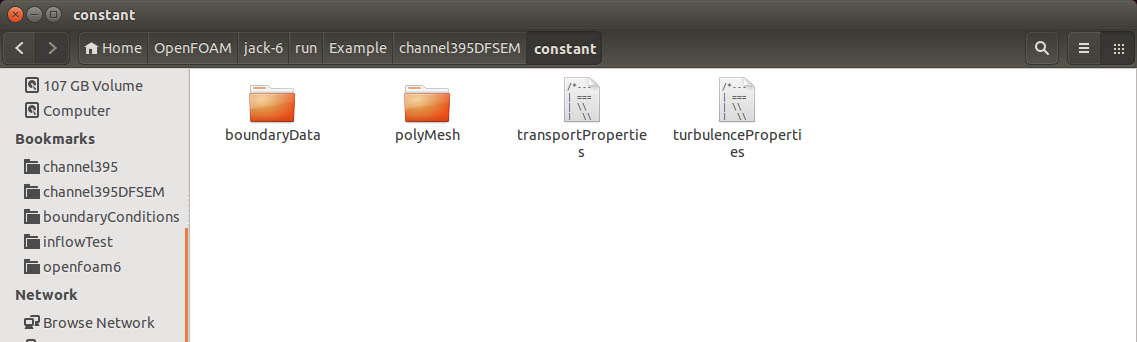
\includegraphics[width=\linewidth]{TInF-theory-01.jpg}
        \caption{the \textcolor{mauve}{``boundaryData"} folder}
     \end{subfigure}
    \begin{subfigure}[b]{\linewidth}
        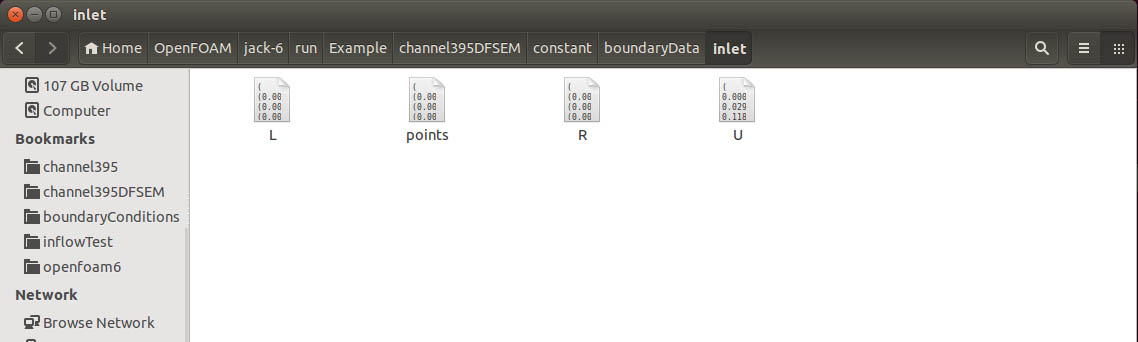
\includegraphics[width=\linewidth]{TInF-theory-02.jpg}
        \caption{the \textcolor{mauve}{``inlet"} folder}
    \end{subfigure}
      \caption{Folders containing the data files for interpolation} \label{folder}
\end{figure}

As mentioned earlier, the source code of the turbulent inflow tool provides some custom-developed boundary conditions for velocities. To implement those boundary conditions during a simulation, there are three files needs to be either modified or created accordingly. These files include: the \textcolor{mauve}{U} file in the \textcolor{mauve}{``0"} folder, the \textcolor{mauve}{inflowProperties} file in the \textcolor{mauve}{``constant"} folder and the \textcolor{mauve}{controlDict} file in the \textcolor{mauve}{``system"} folder. Compared to the \textcolor{mauve}{U} and \textcolor{mauve}{controlDict} files which are required by default in a standard OpenFOAM project, the \textcolor{mauve}{inflowProperties} file is a special item required (when necessary) by the presented boundary conditions. It is designed to store some statistical properties of the target turbulence which include mean velocities, Reynolds stresses and integral length scales.

\subsection{Modifications regarding the \textcolor{mauve}{controlDict} file}

We now introduce the entries or scripts need to be defined in or added to the above mentioned three files respectively. To start with, we consider the \textcolor{mauve}{controlDict} file (inside the \textcolor{mauve}{``system"} folder) and an example of this file is given as follows.

\begin{lstlisting}
/*--------------------------------*- C++ -*----------------------------------*\
  =========                 |
  \\      /  F ield         | OpenFOAM: The Open Source CFD Toolbox
   \\    /   O peration     | Website:  https://openfoam.org
    \\  /    A nd           | Version:  6
     \\/     M anipulation  |
\*---------------------------------------------------------------------------*/
FoamFile
{
    version     2.0;
    format      ascii;
    class       dictionary;
    location    "system";
    object      controlDict;
}
// * * * * * * * * * * * * * * * * * * * * * * * * * * * * * * * * * * * * * //

libs ("libturbulentInflow.so");

application     pisoFoam;

startFrom       startTime;

startTime       0;

stopAt          endTime;

endTime         1;

deltaT          1e-3;

writeControl    timeStep;

writeInterval   100;

purgeWrite      0;

writeFormat     ascii;

writePrecision  6;

writeCompression off;

timeFormat      general;

timePrecision   6;

runTimeModifiable true;

// ************************************************************************* //
\end{lstlisting}

\noindent The only entry needs to be added to this file is the line \textcolor{mauve}{libs(``libturbulentInflow.so")}. This line tells the fluid solver to include the complied library file \textcolor{mauve}{libturbulentInflow.so} prior to the simulation so that the presented boundary conditions contained in this library become available for the current simulation.

\subsection{Modifications regarding the \textcolor{mauve}{U} file}

Subsequently, we focus on the \textcolor{mauve}{U} file located inside the \textcolor{mauve}{``0"} folder. It contains the information of the discrete internal field and boundary fields for the velocity at a specific time instant (see the example given below).

\begin{lstlisting}
/*--------------------------------*- C++ -*----------------------------------*\
  =========                 |
  \\      /  F ield         | OpenFOAM: The Open Source CFD Toolbox
   \\    /   O peration     | Website:  https://openfoam.org
    \\  /    A nd           | Version:  6
     \\/     M anipulation  |
\*---------------------------------------------------------------------------*/
FoamFile
{
    version     2.0;
    format      ascii;
    class       volVectorField;
    object      U;
}
// * * * * * * * * * * * * * * * * * * * * * * * * * * * * * * * * * * * * * //

dimensions      [0 1 -1 0 0 0 0];

internalField   uniform (10 0 0);

boundaryField
{
    inlet
    {
        type            turbulentDFMInlet;
        filterType      exponential;
        gridFactor      1;
        filterFactor    4;
        periodicInY     true;
        periodicInZ     false;
        cleanRestart    false;
        value           $internalField;
    }
    
    inletOld
    {
        type            fixedValue;
        value           uniform (10 0 0);
    }

    outlet
    {
        type            zeroGradient;
    }

    wall
    {
        type            fixedValue;
        value           uniform (0 0 0);
    }
}

// ************************************************************************* //
\end{lstlisting}

\noindent The boundary conditions for velocities are all specified in the \textcolor{mauve}{boundaryField} dictionary, and there are several sub-dictionaries in the \textcolor{mauve}{boundaryField} dictionary with the names such as \textcolor{mauve}{inlet}, \textcolor{mauve}{outlet}, \textcolor{mauve}{wall}, etc. The name of each sub-dictionary corresponds to the name of a particular boundary patch of the mesh, and the entries contained in each sub-dictionary are the related to the boundary condition for the velocity field at the corresponding boundary patch. Let's focus on the sub-dictionary associated with the inflow patch, i.e., the \textcolor{mauve}{inlet} sub-dictionary. The commonly used boundary condition for the velocity at the inflow is the \textcolor{mauve}{fixedValue} condition (see the sub-dictionary \textcolor{mauve}{inletOld}). For a \textcolor{mauve}{fixedValue} velocity boundary, the velocities at the \textcolor{mauve}{inlet} patch are constant and fixed to the vector specified inside the baskets (coming after the \textcolor{mauve}{values} entry) during the simulation. In our case, we would like to the velocities at the \textcolor{mauve}{inlet} patch to be stochastic and time-varying. For this purpose, the developed turbulent inflow package currently provides four boundary conditions in total, i.e. \textcolor{mauve}{turbulentDFMInlet}, \textcolor{mauve}{turbulentSEMInlet}, \textcolor{mauve}{turbulentDFSEMInlet} and \textcolor{mauve}{turbulentATSMInlet}. These four boundary conditions correspond to the synthetic turbulent method by \cite{klein2003}, \cite{jarrin2006}, \cite{poletto2013} and \cite{kroger2018}, respectively.

Also note that each presented boundary condition is, as a matter of fact, a derived class of the \textcolor{mauve}{fixedValue} boundary condition. Since the initialization of the \textcolor{mauve}{fixedValue} boundary condition requires the specification of the \textcolor{mauve}{value} entry. Therefore, this entry should be defined for the four presented boundary conditions as well. However, when one of the four presented boundary conditions is employed, the velocities at the boundary will be later overwritten by the generated turbulence velocity field and consequently the \textcolor{mauve}{value} entry does not have any effect here. Thus, this entry can be just specified as \textcolor{mauve}{{\$}internalField}; Once the \textcolor{mauve}{type} entry takes the \textcolor{mauve}{turbulentDFMInlet}, \textcolor{mauve}{turbulentSEMInlet}, \textcolor{mauve}{turbulentDFSEMInlet} or \textcolor{mauve}{turbulentATSMInlet} boundary condition, there are some unique entries related to each boundary condition accordingly. 

Apart from the \textcolor{mauve}{type} and \textcolor{mauve}{value} entries, there are also some identical entries shared by the four presented boundary conditions. The entries \textcolor{mauve}{periodicInY} and \textcolor{mauve}{periodicInZ} determine whether the synthetic turbulence is periodic in $x_2$ and $x_3$-direction or not, respectively. Before we discuss the \textcolor{mauve}{cleanRestart} entry, it should be mentioned that the four presented boundary conditions are capable of restarting the generation of the synthetic turbulence from an old time-step. This feature is achieved by storing the necessary information and numerical quantities (obtained at the current time-step) which will affect the generation of the turbulence at the next-step. The entry \textcolor{mauve}{cleanRestart} determines whether to disregard those information and generate a new turbulent velocity field at the beginning of a new simulation.

\begin{table}[H]
\centering
\begin{tabular}{c|c|c|c}
\hline
entry name & Type & descriptions & default values \\
\hline
\textcolor{mauve}{periodicInY} & bool & if the synthetic turbulent is periodic in $y$-direction & false \\
\hline
\textcolor{mauve}{periodicInZ} & bool & if the synthetic turbulent is periodic in $z$-direction & false \\
\hline
\textcolor{mauve}{cleanRestart} & bool & whether to disregard old turbulence or not & false \\
\hline
\end{tabular} \caption{Identical entries shared by the four presented boundary conditions}\label{entryIdentical}
\end{table}


\subsubsection{The \textcolor{mauve}{turbulentDFMInlet} boundary condition}

For the \textcolor{mauve}{turbulentDFMInlet} boundary condition, the unique entries to be specified are \textcolor{mauve}{filterType}, \textcolor{mauve}{filterFactor} and \textcolor{mauve}{gridFactor}. The \textcolor{mauve}{filterType} entry refers to the type of the prescribed function for computing the filter coefficients, and requires a string input. When this entry is taken as \textcolor{mauve}{gaussian}, the coefficients are computed with (\ref{gaussian}); when this entry is taken as \textcolor{mauve}{exponential}, the coefficients follow from (\ref{exponential}). As discussed earlier, the digital filtering method should be employed on uniform spacing Cartesian grids. To make this method applies to more general cases, a virtual uniform spacing Cartesian grid system will be generated during the implementation. The velocity fluctuations will be first generated on this virtual grid and then interpolated to the discrete points on the inflow patch. The \textcolor{mauve}{gridFactor} entry defines ratio between the virtual grid spacing $\Delta$ with the square root of the area of the smallest face element on the inflow plane. Higher \textcolor{mauve}{gridFactor} leads to larger grid spacing and vice versa. Finally, the \textcolor{mauve}{filterFactor} entry denotes the values of $N/n$ where $N$ and $n$ follow from the notation in Section \ref{sectionDFM}, and consequently it requires an integer input. The entries related to the turbulentDFMInlet boundary, their input variable types and limitations are listed in Table \ref{entryDigital}.

\begin{table}[H]
\centering
\begin{tabular}{c|c|c|c}
\hline
entry name & Type & limits & default values \\
\hline
\textcolor{mauve}{filterType} & string & gaussian, exponential or bessel & exponential \\
\hline
\textcolor{mauve}{gridFactor} & float & $\geq 1$ & 1 \\
\hline
\textcolor{mauve}{filterFactor} & int & $\geq 4$  & 4 \\
\hline
\end{tabular} \caption{Entries related to the \textcolor{mauve}{turbulentDFMInlet} boundary}\label{entryDigital}
\end{table}

\subsubsection{The \textcolor{mauve}{turbulentSEMInlet} boundary condition}

For the \textcolor{mauve}{turbulentSEMInlet} boundary condition, the unique entries to be specified are \textcolor{mauve}{eddyType} and \textcolor{mauve}{eddyDensity}. The \textcolor{mauve}{eddyType} entry refers to the type of the velocity shape function $f$. It takes a string input and currently the available options are \textcolor{mauve}{tent}, \textcolor{mauve}{step} and \textcolor{mauve}{gaussian} which correspond to (\ref{ftent}), (\ref{fstep}) and (\ref{fgaussian}), respectively. The \textcolor{mauve}{eddyDensity} refers to the ratio between $V_B$ and the sum of the eddy volumes (see Section \ref{sectionSEM}). Higher \textcolor{mauve}{eddyDensity} leads to a larger amount of synthetic eddies. It takes a scalar input with a value no less than one. The lower bound of \textcolor{mauve}{eddyDensity} (taken as 1 by default) ensures the eddy box (introduced in Section \ref{sectionSEM}), from a statistical point of view, can be covered up by eddies. The unique entries for the \textcolor{mauve}{turbulentSEMInlet} condition are summarized in Table \ref{entryEddy}.

\begin{table}[H]
\centering
\begin{tabular}{c|c|c|c}
\hline
entry name & type & limits & default values \\
\hline
\textcolor{mauve}{eddyType} & string & tent, step or gaussian & gaussian \\
\hline
\textcolor{mauve}{eddyDensity} & float & $\geq 1$ & 1 \\
\hline
\end{tabular} \caption{Entries related to the \textcolor{mauve}{turbulentSEMInlet} boundary}\label{entryEddy}
\end{table}

\subsubsection{The \textcolor{mauve}{turbulentDFSEMInlet} boundary condition}

For the \textcolor{mauve}{turbulentDFSEMInlet} boundary condition, the only unique entry to be specified is \textcolor{mauve}{eddyDensity} whose meaning is identical to that of the \textcolor{mauve}{turbulentSEMInlet} boundary condition. 


\subsubsection{The \textcolor{mauve}{turbulentATSMInlet} boundary condition}

For the \textcolor{mauve}{turbulentATSMInlet} boundary condition, the unique entries to be specified are \textcolor{mauve}{vortonType} and \textcolor{mauve}{vortonDensity}. The \textcolor{mauve}{vortonType} entry refers the approach parameter determination for anisotropic vortons discussed in Section \ref{sectionATSM}. It takes an string input and the options currently available are \textcolor{mauve}{typeR} and \textcolor{mauve}{typeL} which correspond to (\ref{fstep}) and (\ref{fgaussian}), respectively. The \textcolor{mauve}{vortonDensity} entry is similar to the \textcolor{mauve}{eddyDensity} of the \textcolor{mauve}{turbulentSEMInlet} boundary condition. We summarize the unique entries for the \textcolor{mauve}{turbulentATSMInlet} condition in Table \ref{entryVorton} for reference.

\begin{table}[H]
\centering
\begin{tabular}{c|c|c|c}
\hline
entry name & type & limits & default values \\
\hline
\textcolor{mauve}{vortonType} & string & typeR or typeL & typeR \\
\hline
\textcolor{mauve}{vortonDensity} & float & $\geq 1$ & 1 \\
\hline
\end{tabular} \caption{Entries related to the \textcolor{mauve}{turbulentATSMInlet} boundary}\label{entryVorton}
\end{table}


\noindent A common feature shared by the entries \textcolor{mauve}{filterFactor}, \textcolor{mauve}{eddyDensity} and \textcolor{mauve}{vortonDensity} mentioned above is that when they are assigned with higher values, the resulting velocity fluctuations will usually have better a quality. However higher values also means a larger consumption of mathematical calculations and computational memory. Therefore, users are suggested to balance the needs between accuracy and efficient during the implementation of those boundary conditions.


\subsection{Specification of the Statistics of the Target Turbulence}

The aforementioned entries defined in the boundary conditions for velocities only concern the selection of the method and the corresponding parameters associated with the selected method. The generation of the synthetic turbulence also requires the statistical information of the target turbulence to be reproduced which include mean velocities, Reynolds stresses and integral length scales. There are mainly three approaches for the input of those information, i.e., \textbf{direct specification}, \textbf{interpolation} and \textbf{prescribed function}.

\subsubsection{Direct Specification}

The direct specification approach is suitable for the case in which the mean velocity, Reynolds stress and length scales on each face element of the inflow plane are known in prior. In this approach, the values of those quantities can be directly specified in the \textcolor{mauve}{inlet} dictionary. If they are uniformly distributed on the inflow plane, the related entries are in the form of

\begin{lstlisting}

boundaryField
{
    inlet
    {
        type            turbulentDFMInlet;
        filterType      exponential;
        gridFactor      1;
        filterFactor    4;
        periodicInY     true;
        periodicInZ     false;
        cleanRestart    false;
        value           $internalField;
        U               uniform 10;
        R               uniform (2.0 0.5 0.5 1.5 -0.5 1.0);
        L               uniform (0.3 0.3 0.3 0.2 0.2 0.2 0.1 0.1 0.1);       
    }
}

\end{lstlisting}

\noindent The three entries displayed in the \textcolor{mauve}{inlet} dictionary are \textcolor{mauve}{U}, \textcolor{mauve}{R} and \textcolor{mauve}{L} which represent mean velocity magnitude, Reynolds stress and length scale. If \textcolor{mauve}{U}, \textcolor{mauve}{R} and \textcolor{mauve}{L} are not uniformly distributed on the inlet patch, the related entries should be defined in the form of

\begin{lstlisting}

boundaryField
{
    inlet
    {
        type            turbulentDFMInlet;
        filterType      exponential;
        gridFactor      1;
        filterFactor    4;
        periodicInY     true;
        periodicInZ     false;
        cleanRestart    false;
        value           $internalField;
        U               
        {
                         1.0
                         2.0
                         ...
                         6.0
        };
        R               
        {
                       (2.0 0.5 0.5 1.5 -0.5 1.0)
                       (2.1 0.6 0.6 1.6 -0.6 1.1)
                       ...
                       (2.5 1.0 1.0 2.0 -1.0 1.5)
        };
        L             
        {
                       (0.30 0.30 0.30 0.20 0.20 0.20 0.10 0.10 0.10)
                       (0.31 0.31 0.31 0.21 0.21 0.21 0.11 0.11 0.11)
                       ...
                       (0.35 0.35 0.35 0.25 0.25 0.25 0.15 0.15 0.15)
        };  
    }
}

\end{lstlisting}

\noindent It is noted that each element in \textcolor{mauve}{R} defines a six-component symmetric tensor of the form ($R_{11}$ $R_{21}$ $R_{31}$ $R_{22}$ $R_{32}$ $R_{33}$). For the \textcolor{mauve}{turbulentDFMInlet} and \textcolor{mauve}{turbulentSEMInlet} boundary conditions, each element in \textcolor{mauve}{L} defines a nine-component tensor of the form ($L_{11}^{x_1}$ $L_{11}^{x_2} \ L_{11}^{x_3}$ $L_{22}^{x_1}$ $L_{22}^{x_2}$ $L_{22}^{x_3}$ $L_{33}^{x_1}$ $L_{33}^{x_2}$ $L_{33}^{x_3}$). For the \textcolor{mauve}{turbulentATSMInlet} boundary condition, each element in \textcolor{mauve}{L} defines a three-component vector of the form ($L_{11}^{x_1}$ $L_{22}^{x_2}$ $L_{33}^{x_3}$).  For the \textcolor{mauve}{turbulentDFSEMInlet} boundary condition, each element in \textcolor{mauve}{L} is a scalar which takes the value of $L_{11}^{x_1}$. The main difficultly in specifying the entries \textcolor{mauve}{U}, \textcolor{mauve}{R} and \textcolor{mauve}{L} directly is to make sure that the sequence of the elements in each entry is properly sorted coping with the corresponding faces on the inflow plane.

\subsubsection{Specification via Interpolation}

The mean velocities, Reynolds stresses and integral length scales on the cell-faces of the inflow plane can also be specified through face interpolation. The detailed procedures are as follows:

\begin{itemize}

\item Create a folder with the name \textcolor{mauve}{``boundaryData"} inside the \textcolor{mauve}{``constant"} folder of a standard OpenFOAM project.

\item Create another folder using the name of the inflow patch inside the above created folder.

\item Add four empty files with the names \textcolor{mauve}{U}, \textcolor{mauve}{R}, \textcolor{mauve}{L} and \textcolor{mauve}{points}, respectively inside the \textcolor{mauve}{inlet} folder. These four files will be used to store the given values of the mean velocity magnitude, Reynolds stress, integral scale at some specific points and the locations of those points in the global coordinate system (of the computational domain).

\item The \textcolor{mauve}{U} file, which stores the information of mean velocity magnitudes, should be written in the format of

\begin{lstlisting} 
(
0.000000
0.029538
0.118110
...
0.029538
0
)
\end{lstlisting}

The entries within the braces are the magnitudes of mean velocity at the corresponding points.

\item The \textcolor{mauve}{R} file, which stores the information of Reynolds stresses, should be written in the format of

\begin{lstlisting} 
(
(0.000000 0.000000 0.000000 0.000000 0.000000 0.000000)
(0.000137 0.000000 0.000000 0.000000 0.000000 0.000053)
(0.002183 0.000002 0.000001 0.000000 0.000000 0.000827)
...
(0.000137 0.000000 0.000000 0.000000 0.000000 0.000053)
(0.000000 0.000000 0.000000 0.000000 0.000000 0.000000)
)
\end{lstlisting}

The entries within the braces are the Reynolds stress tensors at the corresponding points.

\item The \textcolor{mauve}{L} file, which stores the information of turbulence length scales, should be written in the format of

\begin{lstlisting} 
(
(0.000000 0.000000 0.000000 0.000000 0.000000 0.000000 0.000000 0.000000 0.000000)
(0.000024 0.000024 0.000024 0.000024 0.000024 0.000024 0.000024 0.000024 0.000024)
(0.000096 0.000096 0.000096 0.000096 0.000096 0.000096 0.000096 0.000096 0.000096)
...
(0.000024 0.000024 0.000024 0.000024 0.000024 0.000024 0.000024 0.000024 0.000024)
(0.000000 0.000000 0.000000 0.000000 0.000000 0.000000 0.000000 0.000000 0.000000)
)
\end{lstlisting}

The entries within the braces are the components of the turbulence length scales at the corresponding points. Again, both the \textcolor{mauve}{turbulentDFMInlet} and \textcolor{mauve}{turbulentSEMInlet} boundary conditions employ a nine-component length scale. The \textcolor{mauve}{turbulentATSMInlet} and \textcolor{mauve}{turbulentDFSEMInlet} boundary conditions employ a three-component and one-component length scale, respectively.

\item The \textcolor{mauve}{points} file, which stores the locations of the points in the global coordinate system, should be written in the format of

\begin{lstlisting} 
(
(0.000000 0.000000 0.000000)
(0.000000 0.000075 0.000000)
(0.000000 0.000301 0.000000)
...
(0.000000 2.000000 0.000000)
(0.000000 2.000000 3.000000)
)
\end{lstlisting}

It is noted that the points listed in this file should be able to define a single plane. That is to say the points should not locate on a single line or different planes.

\end{itemize}

\noindent In summary, specification of statistics of target turbulent via interpolation is suitable for the case in which the mean velocities, Reynolds stresses and integral length scales at a group of selected points are available.

\subsubsection{Specification via Prescribed Functions} \label{sectionSPF}

Finally, the specification of the mean velocities, Reynolds stresses and integral length scales can also be done with the prescribed functions embedded in the presented boundary conditions. The entries related to this approach are all defined in the \textcolor{mauve}{inflowProperties} file in the \textcolor{mauve}{``constant"} folder. To employ this approach, the first step is to define a local coordinate system and its origin. The local $(x_1',x_2',x_3')$ coordinate system is constructed with its $x_1'$-axis being parallel to normal of the inflow plane and pointing towards the interior of the computational domain.

\begin{figure}[H]
\centering
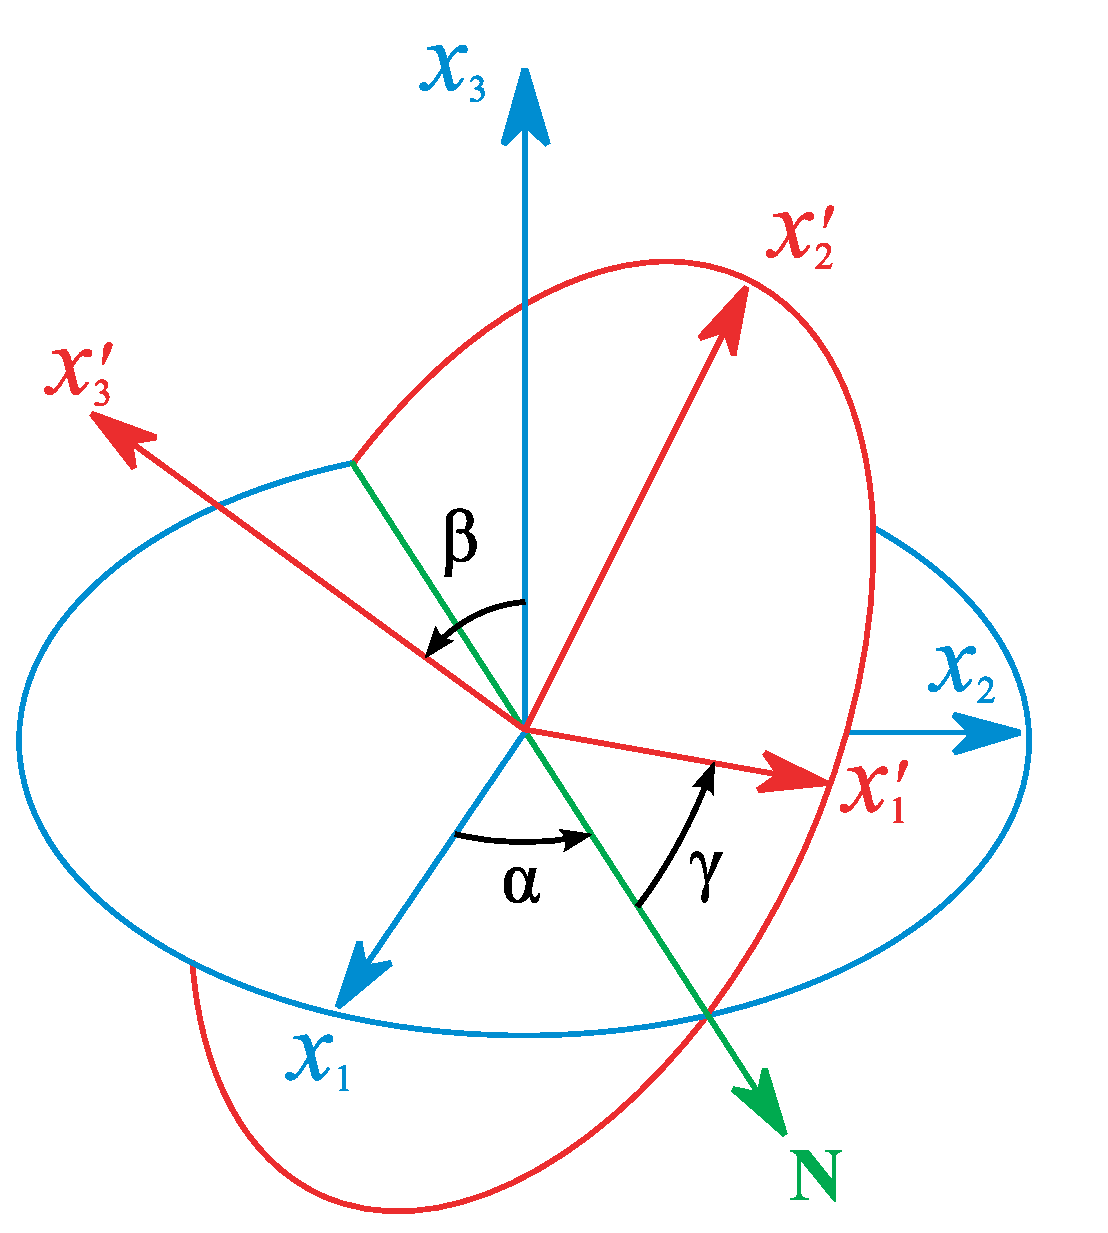
\includegraphics[width=0.3\linewidth]{TInF-theory-03.eps}
\caption{A sketch of the Euler angles and the $N$-axis} \label{EulerAngles}
\end{figure}


To determine the orientation of the $x_2'$- and $x_3'$-axis, an entry named as \textcolor{mauve}{Naxis} is defined which takes a vector input. This vector represents the direction of the $N$-axis (see Fig. \ref{EulerAngles}) where $N$ is the intersection line of the $(x_1',x_2')$-plane and $(x_1,x_2)$-plane. The $x_2'$- and $x_3'$-axis are then determined by $\boldsymbol{x}_2' = \boldsymbol{x}_3'\times\boldsymbol{x}_1'$ and $\boldsymbol{x}_3' = \boldsymbol{x}_1'\times\boldsymbol{N}$. The reason why we specify the direction of the $N$-axis instead of the $x_2'$- or $x_3'$-axis is because, once the direction of the $x_1$-axis is determined, the $x_2'$- and $x_3'$-axis cannot be specified arbitrarily since they must be parallel to the plane orthogonal to the $x_1'$-axis. In contrast, the direction of the $N$-axis can be specified arbitrarily as long as the $x_3$-components of $N$ is zero. The entry \textcolor{mauve}{Naxis} is set as $(0 \ 0 \ 0)$ by default. In this case, the $(x_1',x_2')$-plane and $(x_1,x_2)$-plane are parallel to each other and consequently the $x_3$- and $x_3'$-axis are align.

Now, the remaining issue is the determination of the origin of the local coordinate system. Consider a rectangular defined on the $(x_2',x_3')$-plane bounding all the nodes of the inflow patch. The origin of the local coordinate system is chosen as the lower left corner of this rectangular by default. We also allow users to offset the origin through the use of the entry \textcolor{mauve}{offset} which take a three component vector for input. 

\begin{lstlisting}
/*--------------------------------*- C++ -*----------------------------------*\
  =========                 |
  \      /  F ield         | OpenFOAM: The Open Source CFD Toolbox
   \    /   O peration     | Website:  https://openfoam.org
    \  /    A nd           | Version:  6
     \/     M anipulation  |
\*---------------------------------------------------------------------------*/
FoamFile
{
    version     2.0;
    format      ascii;
    class       dictionary;
    location    "constant";
    object      inflowProperties;
}
// * * * * * * * * * * * * * * * * * * * * * * * * * * * * * * * * * * * * * //

Naxis                  (0 0 0);
offset                 (0 0 0);

UDict
{
    referenceValue          1;
    profile                 uniform;
}

RDict
{
    referenceValue          (0.1  0  0  0.1  0  0.1);
    profile                 uniform;
}

LDict
{
    referenceValue          (0.3 0.2 0.1);
    profile                 uniform;
    Gamma                   (1 1 1);
}

// ************************************************************************* //
\end{lstlisting}

\noindent In addition to the entries mentioned above, there are a total of three sub-dictionaries need to be specified in the \textcolor{mauve}{inflowProperties} file, i.e. \textcolor{mauve}{UDict}, \textcolor{mauve}{RDict} and \textcolor{mauve}{LDict}, which are responsible for the specifications of the mean velocity magnitude, the Reynolds stress tensor $(R_{11}, R_{21}, R_{31}, R_{22}, R_{32}, R_{33})$ and the integral length scales $(L_{11}^{x_1}, L_{22}^{x_2}, L_{33}^{x_3})$. Note $L_{11}^{x_1}$ refers to the integral length scale obtained by integrating the two-point correlation function $R_{11}(\boldsymbol{x})$ with respect to the local $x_1$-direction (i.e., the stream-wise direction) and similarly for $L_{22}^{x_2}$ and $L_{33}^{x_3}$.

Each sub-dictionary contains the entries required for the computation of the values of the corresponding variable on the inlet boundary which are almost identical to each other. In all sub-dictionaries mentioned above, the two basic entries need to be specified are the \textcolor{mauve}{referenceValue} and the \textcolor{mauve}{profile}. For the \textcolor{mauve}{UDict} sub-dictionary, the \textcolor{mauve}{referenceValue} entry requires a scalar value for input, while a symmetric tensor is required for the \textcolor{mauve}{RDict} sub-dictionary. Finally, the \textcolor{mauve}{referenceValue} entry of the \textcolor{mauve}{LDict} sub-dictionary demands a vector.

On the other hand, the \textcolor{mauve}{profile} entry, as its name implies, defines the profile function of the corresponding variable on the inlet boundary. It takes a string variable for input, and there are only two the valid options are \textcolor{mauve}{uniform} and \textcolor{mauve}{exponential} at the present stage (expecting more in the coming future). When the \textcolor{mauve}{profile} entry takes \textcolor{mauve}{uniform}, the corresponding variable will be set universally to the reference value on the entire inflow patch; When the \textcolor{mauve}{profile} entry takes \textcolor{mauve}{exponential}, the corresponding variable will be therefore computed with an exponential function and additional entries entitled as \textcolor{mauve}{alpha}, \textcolor{mauve}{referenceAngl} and \textcolor{mauve}{referenceDist} should be defined as a supplement, see examples below.

\begin{lstlisting}
UDict
{
    referenceValue          1;
    profile                 exponential;
    referenceAngl           0;
    referenceDist           1.0;
    alpha                   0.1;
}

RDict
{
    referenceValue          (0.1  0  0  0.1  0  0.1);
    profile                 exponential;
    referenceAngl           0;
    referenceDist           1.0;
    alpha                   (0.3 0.2 0.1);
}
\end{lstlisting}

\noindent While the entries required for the same type of profile function are almost the same, the form of the exponential function differs in scalar (e.g., the mean velocity magnitude), vector (e.g., the interal length scale) and symmetric tensor variables (e.g., the Reynolds stress tensor). For a scalar variable namely $\phi$, the corresponding exponential function has the form

\begin{equation} \label{exponentialForScalar}
\phi(\boldsymbol{x}) = \bar{\phi}\big(\frac{\boldsymbol{n}\cdot\boldsymbol{x}}{d_0}\big)^{\alpha},
\end{equation}

\noindent where $\bar{\phi}$ is the reference value (defined by the \textcolor{mauve}{referenceValue} entry), $\alpha$ is the exponential coefficient  (defined by the \textcolor{mauve}{alpha} entry), and $d_0$ is a reference distance (defined by the \textcolor{mauve}{referenceDist} entry). The symbol $\boldsymbol{n}$ is a direction vector (located on the inflow plane) to which the spatial coordinate $\boldsymbol{x}$ (defined in the local $(x_1,x_2,x_3)$ coordinate system) is projected. The direction of $\boldsymbol{n}$ is specified indirectly by defining the relative angle between the local $x_3$-axis and $\boldsymbol{n}$, and this angle (ranging from 0 to 180 degrees) is specified in the \textcolor{mauve}{referenceAngl} entry. This reason behind such an approach is obvious, the $\boldsymbol{n}$ can not be arbitrarily specified for it is located on the local $x_1x_2$ (i.e., the inflow) plane. Also for obvious reasons, the reference values of the mean velocity magnitude and integral length scales should be larger than zero.

Similar to scalar variables, for a vector variable namely $\boldsymbol{\phi}=(\phi_1,\phi_2,\phi_3)$, the corresponding exponential function has the form

\begin{equation} \label{exponentialForVector}
\phi_i(\boldsymbol{x}) = \bar{\phi}_i\big(\frac{\boldsymbol{n}\cdot\boldsymbol{x}}{d_0}\big)^{\alpha_i}.
\end{equation}

\noindent where $\boldsymbol{\alpha}=(\alpha_1,\alpha_2,\alpha_3)$ is a vector defined by the \textcolor{mauve}{alpha} entry of vector variables.

Finally a symmetric tensor variable (e.g., the turbulent intensity) denoted by $\boldsymbol{\phi}$ for demonstration, the corresponding exponential function writes

\begin{equation} \label{exponentialForTensor}
\boldsymbol{\phi}(\boldsymbol{x}) = \sum_{\gamma=1}^s \bar{\phi}_{\gamma}\big(\frac{\boldsymbol{n}\cdot\boldsymbol{x}}{d_0}\big)^{\alpha_{\gamma}} \boldsymbol{M}_{\gamma},
\end{equation}

\noindent where $\bar{\phi}_{\gamma}$ ($\gamma=1,2,3$) are principal values of the reference symmetric tensor $\bar{\boldsymbol{\phi}}$ (i.e., the one defined in the \textcolor{mauve}{referenceValue} entry). $\boldsymbol{M}_{\gamma}$ ($\gamma=1,2,3$) are tensors defined by

\begin{equation}
\boldsymbol{M}_{\gamma} = \boldsymbol{a}_{\gamma} \otimes \boldsymbol{a}_{\gamma}
\end{equation}

\noindent where $\boldsymbol{a}_{\gamma}$ are the eigenvectors of $\bar{\boldsymbol{\phi}}$. Other symbols in (\ref{exponentialForTensor}) follow from the notation in (\ref{exponentialForScalar}). Also note that in (\ref{exponentialForTensor}), the \textcolor{mauve}{alpha} entry requires a three-component vector, i.e., $(\alpha_1 \ \alpha_2 \ \alpha_3)$, for input. The \textcolor{mauve}{referenceValue} requires a six-component vector, i.e., $(\bar{\phi}_{11} \ \bar{\phi}_{21} \ \bar{\phi}_{31}\ \bar{\phi}_{22} \ \bar{\phi}_{32}\ \bar{\phi}_{33})$, for input, and for obvious reasons the $\bar{\phi}_{11}$, $\bar{\phi}_{22}$ and $\bar{\phi}_{33}$ components should be larger than zero.


\begin{table}[H]
\centering
\begin{tabular}{c|c|c|c|c}
\hline
\multicolumn{2}{c|}{Entry name} & Type & Limits & Default values \\
\hline
\multirow{3}{*}{referenceValue} & UDict & float & $>0$ & 1 \\
\cline{2-5}
& LDict &  a vector of floats & each entry $>0$ & (1 1 1)\\
\cline{2-5}
& RDict & a vector of floats & the 1\textsuperscript{st}, 4\textsuperscript{th} and 6\textsuperscript{th} entries $>0$  & (1 0 0 1 0 1)\\
\hline
\multicolumn{2}{c|}{profile} & string & uniform or exponential & uniform \\
\hline
\multicolumn{2}{c|}{referenceDist} & float & $>0$ & 1 \\
\hline
\multicolumn{2}{c|}{referenceAngl} & float & between 0 to 180 & 0 \\
\hline
\end{tabular} \caption{Entries listed in the \textcolor{mauve}{inflowProperties} file}\label{entryInflow}
\end{table}